\documentclass[ngerman,a4paper,order=firstname]{../../texmf/tex/latex/mathscript/mathscript}
\usepackage{../../texmf/tex/latex/mathoperators/mathoperators}

\title{\textbf{Lineare Algebra WS2017/18}}
\author{Dozent: Prof. Dr. Arno Fehm}

\begin{document}
\pagenumbering{roman}
\pagestyle{plain}

\maketitle

\hypertarget{tocpage}{}
\tableofcontents
\bookmark[dest=tocpage,level=1]{Inhaltsverzeichnis}

\pagebreak
\pagenumbering{arabic}
\pagestyle{fancy}

\chapter*{Vorwort}
Wir freuen uns, dass du unser Skript für die Vorlesung \textit{Geometrie} bei Prof. Dr. Arno Fehm im WS2018/19 gefunden hast. Da du ja offensichtlich seit einem Jahr Mathematik studierst, kannst du dich glücklich schätzen zu dem einen Drittel zu gehören, dass nicht bis zum zweiten Semester abgebrochen hat.

Wenn du schon das Vorwort zu \textit{Lineare Algebra und analytische Geometrie 1+2} gelesen hast, weißt du sicherlich, dass Prof. Fehm ein Freud der Algebra ist.\footnote{In Zukunft wird sich Prof. Fehm richtig freuen dürfen, denn im Zuge einer neuen Studienordnung, die am 1.4.2019 in Kraft tritt, kommt so gut wie keine Geometrie im \textit{Bachelor Mathematik} vor.} Auf die Frage eines Kommilitonen, wo in seinem Inhaltsverzeichnis (Gruppen, Ringe, Körper) die Geometrie vorkomme, antwortete er:
\begin{quote}
	\textit{Die Frage ist nicht, wieso wir in dieser Vorlesung Algebra statt Geometrie machen, sondern warum hier seit 20 Jahren Geometrie unterrichtet wird.}
\end{quote}

Wie auch im letzten Vorwort können wir dir nur empfehlen die Vorlesung immer zu besuchen, denn dieses Skript ist kein Ersatz dafür. Es soll aber ein Ersatz für deine unleserlichen und (hoffentlich nicht) unvollständigen Mitschriften sein und damit die Prüfungsvorbereitung einfacher machen. Im Gegensatz zu letztem Semester veröffentlicht Prof. Fehm auf seiner Homepage (\url{http://www.math.tu-dresden.de/~afehm/lehre.html}) kein vollständiges Skript mehr, sondern nur noch eine Zusammenfassung.

Der Quelltext dieses Skriptes ist bei Github (\url{https://github.com/henrydatei/TUD_MATH_BA}) gehostet; du kannst ihn dir herunterladen, anschauen, verändern, neu kompilieren, ... Auch wenn wir das Skript immer wieder durchlesen und Fehler beheben, können wir leider keine Garantie auf Richtigkeit geben. Wenn du Fehler finden solltest, wären wir froh, wenn du ein neues Issue auf Github erstellst und dort beschreibst, was falsch ist. Damit wird vielen (und besonders nachfolgenden) Studenten geholfen.

Und jetzt viel Spaß bei \textit{Geometrie}!

\begin{flushright}
	Henry, Pascal und Daniel
\end{flushright}

\chapter{Grundbegriffe der Linearen Algebra}
\section{Logik und Mengen}

\begin{definition}[Teilmenge]
	\proplbl{1_1_8}
	Sind $X$ und $Y$ zwei Mengen, so heißt $X$ eine \begriff{Teilmenge} von 
	$Y$, wenn jedes Element von $X$ auch Element von $Y$ ist, dass heißt wenn für alle 
	$x$ $(x \in X \Rightarrow x \in Y)$ gilt.
\end{definition}

\begin{definition}[Mengenoperationen]
	Seien $X$ und $Y$ Mengen. Man definiert daraus 
	weitere Mengen wie folgt (\begriff{Mengenoperationen}):
	\begin{itemize}
		\item $X \cup Y := \{x \mid x \in X \lor x \in Y\}$
		\item $X \cap Y := \{x \mid x \in X \land x \in Y\}$
		\item $X \backslash Y := \{x \in X \mid x \notin Y\}$
		\item $X \times Y := \{(x,y) \mid x \in X \land y \in Y\}$
		\item $\mathcal P(X) := \{Y \mid Y \subset X\}$
	\end{itemize}
\end{definition}

\section{Abbildungen}

\begin{overview}[Abbildungen]
	Eine \begriff{Abbildung} $f$ von eine Menge $X$ in einer Menge $Y$ ist eine Vorschrift, die jedem $x \in X$
	auf eindeutige Weise genau ein Element $f(x) \in Y$ zuordnet. Man schreibt dies als 
	\begin{align}
	f:
	\begin{cases}
	X \to Y \\ x \mapsto y
	\end{cases}\notag
	\end{align}
	oder $f: X \to Y, x \mapsto y$ oder noch einfacher $f: X \to Y$. Dabei heißt $X$ die
	\begriff{Definitionsmenge} und $Y$ die \begriff{Zielmenge} von $f$. Zwei Abbildungen heißen \begriff[Abbildung!]{gleich}, wenn ihre
	Definitionsmengen und Zielmengen gleich sind und sie jedem $x \in X$ das selbe Element
	$y \in Y$ zuordnen. Die Abbildungen von $X$ nach $Y$ bilden wieder eine Menge, welche wir 
	mit $\Abb(X,Y)$ bezeichnen.
\end{overview}

\begin{example}
	\proplbl{1_2_2}
	\begin{itemize}
		\item Abbildungen mit Zielmenge $\mathbb R$ nennt man Funktion: $f: \mathbb R \to \mathbb
		R, x \mapsto x^2$
		\item Abbildungen mit Zielmenge $\subset$ Definitionsmenge: $f: \mathbb R \to \mathbb
		R_{\le 0}, x \mapsto x^2$ \\
		$\to$ Diese Abbildungen sind verschieden, da sie nicht die selbe Zielmenge haben.
		\item $f: \{0,1\} \to \mathbb R, x \mapsto x^2$
		\item $f: \{0,1\} \to \mathbb R, x \mapsto x$ \\
		$\to$ Diese Funktionen sind gleich. Sie haben die gleichen Definitions- und Zielmengen 
		und sie ordnen jedem Element der Definitionsmenge das gleiche Element der Zielmenge zu.
	\end{itemize}
\end{example}

\begin{example}
	\begin{itemize}
		\item auf jeder Menge $X$ gibt es die \begriff[Abbildung!]{identische Abbildung} (Identität) \\ $\id: X \to X, x 
		\mapsto x$
		\item allgemein kann man zu jeder Teilmenge $A \subset X$ die \begriff[Abbildung!]{Inklusionsabbildung} zuordnen
		$\iota_A: A \to X, x \mapsto x$
		\item zu je zwei Mengen $X$ und $Y$ und einem festen $y_0 \in Y$ gibt es die \begriff[Abbildung!]{konstante
			Abbildung} $c_{y_0}: X \to Y x \mapsto y_0$
		\item zu jder Menge $X$ und Teilmenge $A \subset X$ definiert man die \begriff{charakteristische 
			Funktion}\\ $\chi_A: X \to \mathbb R,
		\begin{cases}
		x \mapsto 1 \quad(x \in A) \\ x \mapsto 0 \quad(x \notin A)
		\end{cases}
		$
		\item zu jeder Menge $X$ gibt es die Abbildung \\ $f: X \times X \to \mathbb R, (x,y) \mapsto
		\delta_{x,y} \begin{cases} 1 \quad (x=y) \\ 0 \quad (x \neq y) \end{cases}$
	\end{itemize}
\end{example}

\begin{definition}[Eigenschaften von Abbildungen]
	Sei $f: X \to Y$ eine Abbildung.
	\begin{enumerate}
		\item $f$ ist \begriff{injektiv},wenn $\forall x,y \in X (f(x) = f(y) \Rightarrow x=y)$.
		\item $f$ ist \begriff{surjektiv}, wenn $\forall y \in Y \exists x \in X (f(x)=y)$ ($\forall n \in N  \exists m \in M \mid f(m)=n$).
		\item $f$ ist \begriff{bijektiv}, wenn $f$ injektiv und surjektiv ist.
	\end{enumerate}
\end{definition}

\begin{example}
	\begin{itemize}
		\item Die identische Abbildung $\id_X:X\to X$ ist stets bijektiv.
		\item Für jede Teilmenge $A\subseteq X$ ist die Inklusionsabbildung $\iota_A:A\to X$ injektiv, aber im Allgemeinen nicht surjektiv.
		\item Die Funktion $f:\real\to\real_{\ge 0}$ mit $x\mapsto x^2$ ist surjektiv, aber nicht injektiv.
		\item Die Funktion $f:\real\to\real$ mit $x\mapsto x^3$ ist bijektiv.
	\end{itemize}
\end{example}

\begin{definition}[Einschränkung]
	\proplbl{1_2_6}
	Sei $f: x \mapsto y$ eine Abbildung. Für $A \subset X$
	definiert man die \begriff{Einschränkung}/\begriff{Restrikton} von $f$ auf $A$ als die Abbildung 
	\begin{align}
		f \vert_A:\begin{cases}
		A \to Y \\ a \mapsto f(a)
		\end{cases}\notag
	\end{align}
	Das \begriff{Bild} von $A$ unter $f$ ist 
	\begin{align}
		f(A) := \{f(a): a \in A\}. \notag
	\end{align}
	Das \begriff{Urbild} einer Menge $B \subset Y$ unter $f$ ist
	\begin{align}
		f^{-1} := \{x \in X: f(x) \in B\}. \notag
	\end{align}
	Man nennt $\Image(f) := f(X)$ das Bild von $f$.
\end{definition}

\begin{remark}
	\proplbl{1_2_7}
	Man ordnet der Abbildung $f: X \to Y$ auch die Abbildungen $\mathcal P(X) \to \mathcal P(Y)$ und
	$\mathcal P(Y) \to \mathcal P(X)$ auf den Potenzmengen zu. Man benutzt hier das gleiche 
	Symbol $f(…)$ sowohl für die Abbildung $f: X \to Y$ als auch für $f: P(X) \to P(Y)$, was 
	unvorsichtig ist, aber keine Probleme bereiten sollte. \\
	In anderen Vorlesungen wird für $y \in Y$ auch $f^{-1}(y)$ statt $f^{-1}(\{y\})$ geschrieben. \\
\end{remark}

\begin{remark}
	\proplbl{1_2_8}
	Genau dann ist $f: X \to Y$ surjektiv, wenn $\Image(f)=Y$ \\
	Genau dann ist $f: X \to Y \begin{cases} $injektiv$ \\ $surjektiv$ \\ $bijektiv$ \end{cases}$, wenn
	$|f^{-1}(\{y\})| = \begin{cases} \le 1 \\ \ge 1 \\ =1  \end{cases} \quad \forall y \in Y$ \\
\end{remark}

\begin{definition}[Komposition]
	Sind $f: X \to Y$ und $g: Y \to Z$ Abbildungen, so ist die
	\begriff{Komposition} $g \circ f$ die Abbildung
	\begin{align}
		g \circ f := \begin{cases}
		X \to Z \\ x \mapsto f(g(x))
		\end{cases}\notag
	\end{align} Man kann 
	die Komposition auffassen als eine Abbildung $\circ: \Abb(Y,Z) \times \Abb(X,Y) \to \Abb(X,Z)$.
\end{definition}

\begin{proposition}
	\proplbl{1_2_10}
	Die Abbildung von Kompositionen ist assoziativ, d.h. es gilt: 
	\begin{align}
		h \circ (g \circ f) = (h \circ g)\circ f\notag
	\end{align}.
\end{proposition}
\begin{proof}
	Sowohl $h\circ (g\circ f)$ als auch $(h\circ g)\circ f$ haben die Definitionsmenge $X$ und die Zielmenge 
	$W$ und für jedes $x\in X$ ist $(h\circ (g\circ f))(x)=h((g\circ f)(x))=h(g(f(x)))=(h\circ g)(f(x)) = 
	((h\circ g)\circ f)(x)$.
\end{proof}

\begin{definition}[Umkehrabbildung]
	Ist $f: X \to Y$ bijektiv, so gibt es zu jedem $y \in Y$
	genau ein $x_y \in X$ mit $f(x_y)=y$ (\propref{1_2_7}), durch 
	\begin{align}
		f^{-1}: \begin{cases}
		Y \to X \\ y \mapsto x_y
		\end{cases}\notag
	\end{align} wird also eine 
	Abbildung definiert, die \begriff{Umkehrabbildung} zu $f$. 
\end{definition}

\begin{proposition}
	Ist die Abbildung $f: X \to Y$ bijektiv, so gelten
	\begin{align}
		f^{-1} \circ f = id_x \notag \\
		f \circ f^{-1} = id_y \notag
	\end{align}
\end{proposition}
\begin{proof}
	Es ist $f^{-1}\in \Abb(X,X)$ und $f\circ f^{-1}\in \Abb(Y,Y)$. Für $y\in Y$ ist $(f\circ f^{-1})(x)=
	f(f^{-1}(y))=y=\id_Y$. Für $x\in X$ ist deshalb $f((f^{-1}\circ f)(x))=(f\circ (f^{-1}\circ f))(x)\overset{\propref{1_2_10}}{=}
	((f\circ f^{-1})\circ f)(x)=(\id_Y \circ f)(x)=f(x)$. Da $f$ injektiv, folgt $f^{-1}\circ f=\id_X$.
\end{proof}

\begin{remark}
	\proplbl{1_2_13}
	Achtung, wir verwenden hier das selbe Symbol $f^{-1}$ für zwei verschiedene Dinge: Die Abbildung
	$f^{-1}: \mathcal P(X) \to \mathcal P(Y)$ aus \propref{1_2_6} existiert für jede Abbildung $f: X \to Y$, aber die
	Umkehrabbildung $f^{-1}: Y \to X$ aus \propref{1_2_10} existiert nur für bijektive Abbildungen $f: X \to Y$.
\end{remark}

\begin{definition}[Familie]
	Seien $I$ und $X$ Mengen. Eine Abbildung $x: I \to X, i \mapsto
	x_i$ nennt man \begriff{Familie} von Elementen von $X$ mit einer Indexmenge I (oder I-Tupel von 
	Elementen von $X$) und schreibt diese auch als $(x_i)_{i \in I}$. Im Fall $I=\{1,2,...,n\}$
	identifiziert man die I-Tupel auch mit den n-Tupeln aus \propref{1_1_8}. Ist $(x_i)_{i \in I}$ eine Familie von
	Teilmengen einer Menge $X$, so ist 
	\begin{itemize}
		\item $\bigcup X_i = \{x \in X \mid \exists i \in I(x \in X)\}$
		\item $\bigcap X_i = \{x \in X \mid \forall i \in I(x \in X)\}$
		\item $\prod X_i = \{f \in \Abb(I,X) \mid \forall i \in I(f(i) \in X_i)\}$
	\end{itemize}
	Die Elemente von $\prod X_i$ schreibt man in der Regel als Familien $(x_i)_{i \in I}$.
\end{definition}

\begin{example}
	Eine Folge ist eine Familie $(x_i)_{i \in I}$ mit der Indexmenge $\mathbb{N}_0$.
\end{example}

\begin{definition}[Graph]
	Der \begriff{Graph} einer Abbildung $f: X \to Y$ ist die Menge
	\begin{align}
		\Gamma f: \{(x,y) \in X \times Y \mid y=f(x)\}\notag
	\end{align}
\end{definition}

\begin{remark}[Formal korrekte Definition einer Abbildung]
	Eine Abbildung $f$ ist ein Tripel $(X,Y,\Gamma)$, wobei $\Gamma \subset X \times Y \quad \forall
	x \in X$ genau ein Paar $(x,y)$ mit $y \in Y$ enthält. Die Abbildungsvorschrift schickt dann
	$x \in X$ auf das eindeutig bestimmte $y \in Y$ mit $(x,y) \in \Gamma$. Es ist dann $\Gamma =
	\Gamma_f$.
\end{remark}

\begin{remark}
	In anderen Vorlesungen wird die Zielmenge nicht immer als Teil der Definition einer Abbildung aufgefasst, d.h. man betrachtet zwei Abbildungen $f:X\to Y$ und $g:X\to Z$ mit gleicher Definitionsmenge dann als gleich, wenn $f(x)=g(x)$ für alle $x\in X$. Dies ist gleichbedeutend mit $\Gamma_f=\Gamma_g$. So würde man dann zum Beispiel $f_1$ und $f_2$ aus \propref{1_2_2} als gleich auffassen.
\end{remark}

\section{Gruppen}

\begin{definition}[(Halb-)Gruppe]
	Sei $G$ eine Menge. Eine (innere, zweistellige) Verknüpfung
	auf $G$ ist eine Abbildung $*: G \times G \to G, (x,y) \mapsto x*y$. Das Paar $(G,*)$ ist eine
	\begriff[Gruppe!]{Halbgruppe}, wenn das folgende Axiom erfüllt ist:
	\begin{itemize}
		\item (G1) Für $x,y,z \in G$ ist $(x*y)*z=x*(y*z)$.
	\end{itemize}
		Eine Halbgruppe $(G,*)$ ist ein \begriff{Monoid}, wenn zusätzlich das folgende Axiom gilt:
	\begin{itemize}
		\item (G2) Es gibt ein Element $e \in G$, welches für alle $x \in G$ die Gleichung $x*e=e*x=x$
		erfüllt. Dieses Element heißt dann \begriff{neutrales Element} der Verknüpfung $*$.  
	\end{itemize}
\end{definition}

\begin{example}
	\begin{itemize}
		\item Für jede Menge $X$ ist $(\Abb(X,Y), \circ)$ eine Halbgruppe (\propref{1_2_10}) mit dem neutralen Element
		$\id_x$, also ein Monoid.
		\item $\mathbb N$ bildet mit der Addition eine Halbgruppe $(\mathbb N,+)$, aber kein Monoid,
		da die 0 nicht in Fehm's Definition der natürlichen Zahlen gehörte
		\item $\mathbb N_0$ bildet mit der Addition ein Monoid $(\mathbb N_0,+)$
		\item $\mathbb N$ bildet mit der Multiplikation ein Monoid $(\mathbb N, \cdot)$
		\item $\mathbb Z$ bildet mit der Multiplikation ein Monoid $(\mathbb Z, \cdot)$
	\end{itemize}
\end{example}

\begin{proposition}[Eindeutigkeit des neutralen Elements]
	Ein Monoid $(G,*)$ hat genau ein neutrales Element. 
\end{proposition}
\begin{proof}
	Nach Definition besitzt $(G,*)$ mindestens ein neutrales Element. Seien $e_1,e_2\in G$ neutrale Elemente. Dann 
	ist $e_1=e_1 * e_2=e_2$. Damit besitzt $(G,*)$ höchstens ein neutrales Element, also genau ein neutrales Element.
\end{proof}

\begin{definition}[(abelsche) Gruppe]
	Eine \begriff{Gruppe} ist ein Monoid $(G,*)$ mit dem neutralen Element
	$e$, in dem zusätzlich das folgende Axiom gilt:
	\begin{itemize}
		\item (G3) Für jedes $x \in G$ gibt es ein $x' \in G$ mit $x'*x=x*x'=e$.
	\end{itemize}
	Gilt weiterhin
	\begin{itemize}
		\item (G4) Für alle $x,y \in G$ gilt $x*y=y*x$, so heißt diese Gruppe \begriff[Gruppe!]{abelsch}.
	\end{itemize}
\end{definition}

Ein $x'$ heißt \begriff{inverses Element} zu $x$. \\

\begin{example}
	\begin{itemize}
		\item $\mathbb N_0$ bildet mit der Addition keine Gruppe $(\mathbb N_0,+)$
		\item $\mathbb Z$ bildet mit der Addition eine abelsche Gruppe $(\mathbb Z,+)$
		\item Auch $(\mathbb Q,+)$ und $(\mathbb R,+)$ sind abelsche Gruppen
		\item $(\mathbb Q,\cdot)$ ist keine Gruppe, aber $(\mathbb Q\backslash\{0\},\cdot)$ schon
	\end{itemize}
\end{example}

\begin{proposition}[Eindeutigkeit des Inversen]
	Ist $(G,*)$ eine Gruppe, so hat jedes $x \in G$ genau ein inverses Element.
\end{proposition}
\begin{proof}
	Nach Definition hat jedes $x\in G$ mindestens ein Inverses. Seien $x',x''\in G$ inverse Elemente zu $x$. Dann ist 
	$x'=x'*e=x'*(x*x'')=(x'*x)*x''=e*x''=x''$. Es gibt also genau ein Inverses zu $x$.
\end{proof}

\begin{example}
	\proplbl{1_3_7}
	\begin{itemize}
		\item Eine triviale Gruppe besteht nur aus ihrem neutralen Element. Tatsächlich ist $G=\{e\}$ mit
		$e*e=e$ eine Gruppe.
		\item Sei $X$ eine Menge. Die Menge $\Sym(X) := \{f \in \Abb(X,X) \mid f$ ist bijektiv$\}$ der
		Permutationen von $X$ bildet mit der Komposition eine Gruppe $(\Sym(X),\circ)$, die 
		\begriff[Gruppe!]{symmetrische Gruppe} auf $X$. Für $n \in \mathbb N$ schreibt man $S_n := \Sym(\{1,2,...,n\})$. 
		Für $n \ge 3$ ist $S_n$ nicht abelsch.
	\end{itemize}
\end{example}

\begin{remark}
	Häufig benutzte Notationen für die Gruppenverknüpfung $\cdot$:
	\begin{itemize}
		\item In der multiplikativen Notation schreibt man $\cdot$ statt $*$ (oft auch $xy$ statt 
		$x \cdot y$), bezeichnet das neutrale Element mit $1$ oder $1_G$ und das Inverse zu $x$ mit
		$x^{-1}$.
		\item In der additiven Notation schreibt man $+$ für $*$, bezeichnet das neutrale Element
		mit $0$ oder $0_G$ und das Inverse zu $x$ mit $-x$. Die additive Notation wird nur verwendet,
		wenn die Gruppe abelsch ist.
	\end{itemize}
\end{remark}

In abelschen Gruppen notiert man Ausdrücke auch mit dem Summen- und Produktzeichen. \\

\begin{proposition}
	Sei $(G,\cdot)$ eine Gruppe. Für $x,y \in G$ gelten
	\begin{align}
		(x^{-1})^{-1} &= x \notag \\
		(xy)^{-1} &= x^{-1} \cdot y^{-1} \notag
	\end{align}
\end{proposition}
\begin{proof}
	Nach Definition erfüllt $z=x$ die Identitäten $x^{-1}z=zx^{-1}=1$ und somit ist $(x^{-1})^{-1}=z=x$. Ebenso ist 
	$(y^{-1}x^{-1})\cdot (xy)=y^{-1}(x^{-1}x)y=1$ und $(xy)\cdot (x^{-1}y^{-1})=x(yy^{-1})x^{-1}=1$, also $y^{-1}
	x^{-1}=(xy)^{-1}$.
\end{proof}

\begin{proposition}
	\proplbl{1_3_10}
	Sei $(G,\cdot)$ eine Gruppe. Für $a,b \in G$ haben die Gleichungen $ax=b$ und
	$ya=b$ eindeutige Lösungen in $G$, nämlich $x=a^{-1} \cdot b$ und $y=b \cdot a^{-1}$. 
	Insbesondere gelten die folgenden Kürzungsregeln: $ax=ay \Rightarrow x=y$ und $xa=ya 
	\Rightarrow x=y$.
\end{proposition}
\begin{proof}
	Es ist $a \cdot a^{-1} \cdot b = 1b=b$, also ist $x=a^{-1} \cdot b$ eine Lösung. Ist umgekehrt
	$ax=b$ mit $x \in G$, so ist $a^{-1} \cdot b = a^{-1} \cdot ax = 1x = x$ die Lösung und somit
	eindeutig. Für die zweite Gleichung argumentiert man analog. Den "'Insbesondere"'-Fall erhält
	man durch Einsetzen von $b=ay$ bzw. $b=xa$.
\end{proof}

\begin{remark}
	Wenn aus dem Kontext klar ist, welche Verknüpfung gemeint ist, schreibt man auch einfach
	$G$ anstatt $(G, \cdot)$ bzw. $(G,+)$. Eine Gruppe $G$ heißt endlich, wenn die Menge $G$ endlich
	ist. Die Mächtigkeit $|G|$ von $G$ nennt man dann die Ordnung von $G$. Eine endliche Gruppe kann 
	durch ihre Verknüpfungstafel vollständig beschrieben werden.
\end{remark}

\begin{example}
	\begin{itemize}
		\item die triviale Gruppe $G=\{e\}$
		\begin{center}
			\begin{tabular}{|c|c|}
				\hline
				$\cdot$ & $e$\\
				\hline
				$e$ & $e$ \\
				\hline
			\end{tabular}
		\end{center}
		\item die Gruppe $\mu_2 = \{1,-1\}$ der Ordnung 2
		\begin{center}
			\begin{tabular}{|c|c|c|}
				\hline
				$\cdot$ & $1$ & $-1$\\
				\hline
				$1$ & $1$ & $-1$ \\
				\hline
				$-1$ & $-1$ & $1$ \\
				\hline
			\end{tabular}
		\end{center}
		\item die Gruppe $S_2= \Sym(\{1,2\}) = \{\id_{\{1,2\}},f\}$, wobei $f(1)=2$ und $f(2)=1$
		\begin{center}
			\begin{tabular}{|c|c|c|}
				\hline
				$\circ$ & $\id_{\{1,2\}}$ & $f$\\
				\hline
				$\id_{\{1,2\}}$ & $\id_{\{1,2\}}$ & $f$ \\
				\hline
				$f$ & $f$ & $\id_{\{1,2\}}$ \\
				\hline
			\end{tabular}
		\end{center}
	\end{itemize}
\end{example}

\begin{definition}[Untergruppe]
	Eine \begriff{Untergruppe} einer Gruppe $(G,\cdot)$ ist eine 
	nichtleere Teilmenge $H \subset G$, für die gilt:
	\begin{itemize}
		\item (UG1) Für alle $x,y \in H$ ist $x \cdot y \in H$ (Abgeschlossenheit unter Multiplikation).
		\item (UG2) Für alle $x \in H$ ist $x^{-1} \in H$ (Abgeschlossenheit unter Inversen).
	\end{itemize}
\end{definition}

\begin{proposition}
	\proplbl{1_3_14}
	Sei $(G,\cdot)$ eine Gruppe und $\emptyset \neq H \subset G$. Genau dann ist
	$H$ eine Untergruppe von $G$, wenn sich die Verknüpfung $\cdot: G \times G \to G$ zu einer
	Abbildung $\cdot_H: H \times H \to H$ einschränken lässt (d.h. $\cdot\vert_{H \times H}=
	\iota_H \circ \cdot_H$, wobei $\iota_H \cdot \cdot_H \to G$ die Inklusionsabbildung ist) und
	$(H,\cdot_H)$ eine Gruppe ist.
\end{proposition}
\begin{proof}
	$\Rightarrow$: Sei $H$ eine Untergruppe von $G$. Nach (UG1) ist $\Image(\cdot|_{H \times H}) \subset H$
	und somit lässt sich $\cdot$ zu einer Abbildung $\cdot_H: H \times H \ to H$ einschränken. Wir 
	betrachten jetzt $H$ mit dieser Verknüpfung. Da $G$ (G1) erfüllt, erfüllt auch H (G1). Da
	$H \neq \emptyset$ existiert ein $x \in H$. Nach (UG1) und (UG2) ist $x \cdot x^{-1}=e \in H$. Da 
	$e_G \cdot y=y \cdot e_G=y$ für alle $y \in G$, insbesondere auch für alle $y \in H$ (G2). Wegen
	(UG2) erfüllt $H$ auch das Axiom (G3). $H$ ist somit eine Gruppe. \\
	$\Leftarrow$: Sei nun umgekehrt $(H,\cdot_H)$ eine Gruppe. Für $x,y \in H$ ist dann $xy=x \cdot_H
	y \in H$, also erfüllt $H$ (UG1). Aus $e_H \cdot e_H=e_H=e_H \cdot e_G$ folgt $e_H=e_G$. Ist also
	$x'$ das Inverse zu $x$ aus der Gruppe $H$, so ist $x'x=xx'=e_G=e_H$, also $x^{-1}=x' \in H$ und
	somit erfüllt $H$ auch (UG2). Wir haben gezeigt, dass $H$ eine Untergruppe von $G$ ist.
\end{proof}

\begin{remark}
	Wir nennen nicht nur die Menge $H$ eine Untergruppe von $G$, sondern auch die Gruppe $(H,\cdot_H)$.
	Wir schreiben $H \subseteq G$.
\end{remark}

\begin{example}
	\proplbl{1_3_16}
	\begin{itemize}
		\item Jede Gruppe $G$ hat die triviale Untergruppe $H=\{e_G\}$ und $H=G$
		\item Ist $H \subseteq G$ und $K \subseteq H$, so ist $K \subseteq G$ (Transitivität)
		\item Unter Addition ist $\mathbb{Z} \subseteq \mathbb{Q} \subseteq \mathbb{R}$ eine Kette von Untergruppen
		\item Unter Multiplikation ist $\mu_2 \subseteq \mathbb{Q}^+ \subseteq \mathbb{R}^+$ eine Kette von 
		Untergruppen
		\item Für $n \in \mathbb{N}_0$ ist $n\mathbb{Z} := \{nx \mid x \in \mathbb{Z}\} \subseteq \mathbb{Z}$ 
	\end{itemize}
\end{example}

\begin{lemma}
	\proplbl{1_3_17}
	Ist $G$ eine Gruppe und $(H_i)_{i \in I}$ eine Familie von Untergruppen von $G$,
	so ist auch $H := \bigcap H_i$ eine Untergruppe von $G$.
\end{lemma}
\begin{proof}
	Wir haben 3 Dinge zu zeigen
	\begin{itemize}
		\item $H \neq \emptyset:$ Für jedes $i \in I$ ist $e_G \in H$, also auch $e_G \in \bigcap
		H_i =H$
		\item (UG1): Seien $x,y \in H$. Für jedes $i \in I$ ist $x,y \in H_i$, somit $xy \in H_i$,
		da $H_i \subseteq G$. Folglich ist $xy \in \bigcap H_i=H$.
		\item (UG2): Sei $x \in H$. Für jedes $i \in I$ ist $x \in H_i$, somit $x^{-1} \in H_i$,
		da $H_i \subseteq G$. Folglich ist $x^{-1} \in \bigcap H_i=H$.
	\end{itemize}
\end{proof}

\begin{proposition}
	Ist $G$ eine Gruppe und $X \subset G$. so gibt es eine eindeutig bestimmte
	kleinste Untergruppe $H$ von $G$, die $X$ enthält, d.h. $H$ enthält $X$ und ist $H'$
	eine weitere Untergruppe von $G$, die $X$ enthält, so ist $H \subset H'$.
\end{proposition}
\begin{proof}
	Sei $\mathcal{H}$ die Menge aller Untergruppen von $G$, die $X$ enthalten. Nach \propref{1_3_17}
	ist $H:=
	\bigcap \mathcal{H} := \bigcap H$ eine Untergruppe von $G$. Da $X \subset H'$ für jedes $H' \in 
	\mathcal H$ ist auch $X \subset H$. Nach Definition ist $H$ in jedem $H' \subseteq G$ mit $X \subset H'$
	enhalten.
\end{proof}

\begin{definition}[erzeugte Untergruppe]
	Ist $G$ eine Gruppe und $X \subseteq G$, so nennt man diese
	kleinste Untergruppe von $G$, die $X$ enthält, die von $X$ \begriff[Untergruppe!]{erzeugte Untergruppe} von $G$ und
	bezeichnet diese mit $\langle X\rangle$, falls $X = \{x_1,x_2,...,x_n\}$ enthält auch mit $\langle x_1,x_2,
	...,x_n\rangle$. Gibt es eine endliche Menge $X \subset G$ mit $G=\langle X\rangle$, so nennt man $G$ endlich
	erzeugt.
\end{definition}

\begin{example}
	\begin{itemize}
		\item Die leere Menge $X=\emptyset \subseteq G$ erzeugt stets die triviale Untergruppe $\langle \emptyset\rangle
		=\{e\} \subseteq G$
		\item Jede endliche Gruppe $G$ ist endlich erzeugt $G=\langle G\rangle$
		\item Für $n \in \mathbb{N}_0$ ist $n\mathbb{Z}=\langle n\rangle \subseteq \mathbb{Z}$. Nach \propref{1_3_16} ist $n\in n\whole\subseteq\whole$. Ist $H \subseteq \mathbb{Z}$
		mit $n \in H$, so ist auch $kn=nk=n+n+...+n \in H$ und somit auch $n\mathbb{Z} \subseteq H$.
	\end{itemize}
\end{example}

\section{Ringe}

\begin{definition}[Ring]
	Ein \begriff{Ring} ist ein Tripel $(R,+,\cdot)$ bestehend aus einer Menge
	$R$, einer Verknüpfung $+: R \times R \to R$ (Addition) und einer anderen Verknüpfung
	$\cdot: R \times R \to R$ (Multiplikation), sodass diese zusammen die folgenden Axiome 
	erfüllen:
	\begin{itemize}
		\item (R1) $(R,+)$ ist eine abelsche Gruppe.
		\item (R2) $(R,\cdot)$ ist eine Halbgruppe.
		\item (R3) Für $a,x,y \in R$ gelten die Distributivgesetze $a(x+y)=ax+ay$ und $(x+y)a=xa+ya$.
	\end{itemize}
	Ein Ring heißt kommutativ, wenn $xy=yx$ für alle $x,y \in R$.\\
	Ein neutrales Element der Multiplikation heißt Einselement von $R$.\\
	Ein Unterring eines Rings $(R,+,\cdot)$ ist eine Teilmenge, die mit der geeigneten
	Einschränkung von Addition und Multiplikation wieder ein Ring ist.
\end{definition}

\begin{remark}
	Hat ein Ring ein Einselement, so ist dieses eindeutig bestimmt. Notationelle Konfektionen: Das 
	neutrale Element der Addition wird häufig mit 0 bezeichnet; die Multiplikation wird nicht immer
	notiert; Multiplikation bindet stärker als die Addition. \\
	Wenn die Verknüpfungen aus dem Kontext klar sind, schreibt ma $R$ statt $(R,+,\cdot)$.
\end{remark}

\begin{example}
	\begin{itemize}
		\item Der Nullring ist $R=\{0\}$ mit den einzig möglichen Verknüpfungen $+$ und $\cdot$
		auf $R$. Der Nullring ist sogar kommutativ und hat ein Einselement, nämlich die 0.
		\item $(\mathbb{Z},+,\cdot)$ ist ein kommutativer Ring mit Einselement 1, ebenso
		$(\mathbb{Q},+,\cdot)$ und $(\mathbb{R},+,\cdot)$. 
		\item $(2\mathbb{Z},+,\cdot)$ ist ein kommutativer Ring, aber ohne Einselement.
	\end{itemize}
\end{example}

\begin{remark}
	Ist $R$ ein Ring, dann gelten die folgenden Aussagen für $x,y \in R$
	\begin{itemize}
		\item $0 \cdot x=x \cdot 0 = 0$
		\item $x \cdot (-y) = (-x) \cdot y = -xy$
		\item $(-x) \cdot (-y) = xy$
	\end{itemize}
\end{remark}

\begin{remark}
	Wir führen eine wichtige Klasse endlicher Ringe ein. Hierfür erinnern wir uns an eine der Grundlagen
	der Arithmetik in $\mathbb{Z}$.
\end{remark}

\begin{theorem}
	\proplbl{1_4_6}
	Sei $b \neq 0 \in \mathbb{Z}$. Für jedes $a \in \mathbb{Z}$ gibt es 
	eindeutig bestimmte $q,r \in \mathbb{Z}$ ($r$ ist "'Rest"'), mit $a=qb+r$ und $0 \le r < \vert b\vert$.
\end{theorem}
\begin{proof}
	Existenz und Eindeutigkeit
	\begin{itemize}
		\item Existenz: oBdA nehmen wir an, dass $b>0$ (denn ist $a=qb+r$, so ist auch $a=(-q)(-b)+r$). Sei $q \in
		\mathbb{Z}$ die größte Zahl mit $q \le \frac{a}{b}$, und sei $r=a-qb \in \mathbb{Z}$. Dann ist
		$a \le \frac{a}{b}-q < 1$, woraus $0 \le r < b$ folgt.
		\item Eindeutigkeit: Sei $a=qb+r=q'b+r'$ mit $q,q',r,r' \in \mathbb{Z}$ und $0 \le r,r' < |b|$. Dann ist
		$(q-q')b=r-r'$ und $|r-r'|<|b|$. Da $q-q' \in \mathbb{Z}$ ist, folgt $r-r'=0$ und daraus wegen 
		$b \neq 0$, dann $q-q'=0$.
	\end{itemize}
\end{proof}

\begin{example}[Restklassenring]
	Wir fixieren $n \in \mathbb{N}$. Für $a \in \mathbb{Z}$ sei
	$\overline{a} := a+n\mathbb{Z} := \{a+nx \mid x \in \mathbb{Z}\}$ die \begriff{Restklasse} von "$a \bmod n$". 
	Für $a,a' \in \mathbb{Z}$ sind äquivalent:
	\begin{itemize}
		\item $a+n\mathbb{Z}=a'+n\mathbb{Z}$
		\item $a' \in a+n\mathbb{Z}$
		\item $n$ teilt $a'-a$ (in Zeichen $n|a'-a$), d.h. $a'=a+nk$ für $k \in \mathbb{Z}$
	\end{itemize}
\end{example}
\begin{proof}
	\begin{itemize}
		\item $1) \Rightarrow 2)$: klar, denn $0 \in \mathbb{Z}$
		\item $2) \Rightarrow 3)$: $a' \in a+n\mathbb{Z} \Rightarrow a'=a+nk$ mit $k \in \mathbb{Z}$
		\item $3) \Rightarrow 1)$: $a'=a+nk$ mit $k \in \mathbb{Z} \Rightarrow a+n\mathbb{Z}=\{a+nk+nx \mid 
		x \in \mathbb{Z}\}=\{a+n(k+x) \mid x \in \mathbb{Z}\}=a+n\mathbb{Z}$
	\end{itemize}
	Insbesondere besteht $a+n\mathbb{Z}$ nur aus den ganzen Zahlen, die bei der Division durch $n$ den selben Rest lassen wie $a$.
\end{proof}

Aus \propref{1_4_6} folgt weiter, dass $\mathbb{Z}/n\mathbb{Z} := \{\overline{a} \mid a \in \mathbb{Z}\}
= \{\overline{0}, \overline{1},..., \overline{n-1}\}$ eine Menge der Mächtigkeit n ist (sprich: 
"'$\mathbb{Z} \bmod n\mathbb{Z}$"'). \\
$\newline$

Wir definieren Verknüpfungen auf $\mathbb{Z}/n\mathbb{Z}$ durch $\overline{a}+\overline{b} :=
\overline{a+b}$, $\overline{a} \cdot \overline{b} := \overline{ab}$ $a,b \in \mathbb{Z}$. Hierbei
muss man zeigen, dass diese Verknüpfungen wohldefiniert sind, also nicht von den gewählten
Vertretern $a,b$ der Restklassen $\overline{a}$ und $\overline{b}$ abhängen. Ist etwa $\overline{a}
= \overline{a'}$ und $\overline{b}= \overline{b'}$, also $a'=a+nk_1$ und $b'=b+nk_2$ mit $k_1,k_2 \in
\mathbb{Z}$, so ist \\
$a'+b' = a+b+n(k_1+k_2)$, also $\overline{a'+b'} = \overline{a+b}$ \\
$a' \cdot b' = ab+n(bk_1+ak_2+nk_1k_2)$, also $\overline{a'b'} = \overline{ab}$ \\
Man prüft nun leicht nach, dass $\mathbb{Z}/n\mathbb{Z}$ mit diesen Verknüpfungen ein kommutativer
Ring mit Einselement ist, da dies auch für $(\mathbb{Z},+,\cdot)$ gilt. Das neutrale Element der
Addition ist $\overline{0}$, das Einselement ist $\overline{1}$. \\
$\newline$

\begin{example}
	Im Fall $n=2$ ergeben sich die folgenden Verknüpfungstafeln für $\mathbb{Z}
	/2\mathbb{Z} = \{\overline{0}, \overline{1}\}$ \\
	\begin{center}
		\begin{tabular}{|c|c|c|}
			\hline
			$+$ & $\overline{0}$ & $\overline{1}$\\
			\hline
			$\overline{0}$ & $\overline{0}$ & $\overline{1}$\\
			\hline
			$\overline{1}$ & $\overline{1}$ & $\overline{2}=\overline{0}$ \\
			\hline
		\end{tabular}
	\end{center}
	\begin{center}
		\begin{tabular}{|c|c|c|}
			\hline
			$\cdot$ & $\overline{0}$ & $\overline{1}$\\
			\hline
			$\overline{0}$ & $\overline{0}$ & $\overline{0}$\\
			\hline
			$\overline{1}$ & $\overline{0}$ & $\overline{1}$ \\
			\hline
		\end{tabular}
	\end{center}
\end{example}

\begin{definition}[Charakteristik]
	Sei $R$ ein Ring mit Einselement. Man definiert die \begriff{Charakteristik} von
	$R$ als die kleinste natürliche Zahl $n$ mit $1+1+...+1=0$, falls so ein $n$ existiert, andernfalls
	ist die Charakteristik $0$.
\end{definition}

\begin{definition}[Nullteiler]
	Sei $R$ ein Ring mit Einselement. Ein $0 \neq x \in R$ ist ein \begriff{Nullteiler} von 
	$R$, wenn er ein $0 \neq y \in R$ mit $xy=0$ oder $yx=0$ gibt. Ein Ring ohne Nullteiler ist
	nullteilerfrei.
\end{definition}

\begin{definition}[Einheit]
	Sei $R$ ein Ring mit Einselement. Ein $x \in R$ heißt invertierbar (oder
	\begriff{Einheit} von $R$), wenn es ein $x' \in R$ mit $xx'=x'x=1$ gibt. Wir bezeichnen die invertierten
	Elemente von $R$ mit $R^{\times}$.
\end{definition}

\begin{example}
	\proplbl{1_4_12}
	\begin{itemize}
		\item reelle Zahlen sind ein nullteilerfreier Ring der Charakteristik $0$ mit $\mathbb R^{\times}=
		\mathbb R\backslash\{0\}$
		\item $\mathbb Z$ ist ein nullteilerfreier Ring der Charakteristik $0$ mit $\mathbb Z^{\times}=
		\{1,-1\}$
		\item $\mathbb Z/n \mathbb Z$ ist ein Ring der Charakteristik $n$. Ist $n$ keine Primzahl, so
		ist $\mathbb Z$ nicht nullteilerfrei.
	\end{itemize}
\end{example}

\begin{proposition}
	\proplbl{1_4_13}
	Sei $R$ ein Ring mit Einselement. 
	\begin{itemize}
		\item Ist $x \in R$ invertierbar, so ist $x$ kein Nullteiler in $R$.
		\item Die invertierbaren Elemente von $R$ bilden mit der Multiplikation eine Gruppe.
	\end{itemize}
\end{proposition}
\begin{proof}
	\begin{itemize}
		\item Ist $xx'=x'x=1$ und $xy=0$ mit $x',y \in R$, so ist $0=x'\cdot 0=x\cdot xy=1\cdot y=y$, aber
		$y \neq 0$ für Nullteiler
		\item Sind $x,y \in R^{\times}$, also $xx'=x'x=yy'=y'y=1$. Dann ist $(xy)(y'x')=x\cdot 1\cdot x'=1$
		und $(y'x')(xy)=y'\cdot 1\cdot y=1$, somit $R^{\times}$ abgeschlossen unter der Multiplikation. Da 
		$1 \cdot 1=1$ gilt, ist auch $1 \in R^{\times}$. Nach Definition von $R^{\times}$ hat jedes $x \in 
		R^{\times}$ ein Inverses $x' \in R^{\times}$.
	\end{itemize}
\end{proof}
\section{Körper}

\begin{definition}[Körper]
	Ein \begriff{Körper} ist ein kommutativer Ring $(K,+,\cdot)$ mit Einselement 
	$1 \neq 0$, in dem jedes Element $x \neq x \in K$ invertierbar ist.
\end{definition}

\begin{definition}[Teilkörper]
	Ein \begriff{Teilkörper} eines Körpers $(K,+,\cdot)$ ist die Teilemenge $L 
	\subset K$, die mit der geeigneten Einschränkung von Addition und Multiplikation wieder ein
	Körper ist.
\end{definition}

\begin{example}[Endliche Primkörper]
	Für jede Primzahl $p$ ist $\mathbb Z /p \mathbb Z$ ein Körper. Ist $\overline{a}\neq \overline{0}$, so gilt 
	$p$ teilt nicht $a$ und somit gibt es nach \propref{1_5_7} $b,k \in \mathbb Z$ mit \\
	\begin{align}
		ab+kp &= 1 \notag \\
		\overline{(ab+kp)} &= \overline{1} = \overline{(ab)} = \overline{a} \cdot \overline{b} \notag
	\end{align}
	und somit ist $\overline{a}$ invertierbar in $\mathbb Z /p \mathbb Z$. Somit sind für $n \in \mathbb N$
	äquivalent:
	\begin{itemize}
		\item $\mathbb Z /n \mathbb Z$ ist ein Körper
		\item $\mathbb Z /n \mathbb Z$ ist nullteilerfrei
		\item $n$ ist Primzahl
	\end{itemize}
\end{example}
\begin{proof}
	\begin{itemize}
		\item 1 $\Rightarrow$ 2: \propref{1_4_13}
		\item 2 $\Rightarrow$ 3: \propref{1_4_12}
		\item 3 $\Rightarrow$ 1: gegeben
	\end{itemize}
	Insbesondere ist $\mathbb Z /p \mathbb Z$ nullteilerfrei, d.h. aus $p\vert ab$ folgt $p\vert a$ oder $p\vert b$.
\end{proof}
\section{Polynome}

In diesem Abschnitt sei $R$ ein kommutativer Ring mit Einselement.\\

\begin{definition}[Polynom]
	Sei $R[X]$ die Menge der Folgen in $R$ (siehe \propref{1_2_13}), die fast überall 0 sind, also
	\begin{align}
		R[X]:=\{(a_k)_{k \in \mathbb N_0} \mid \forall k(a_k \in R) \land \exists n_0: \forall k>n_0(a_k=0)\} \notag
	\end{align}
\end{definition}

Wir definieren Addition und Multiplikation auf $R[X]$:
\begin{itemize}
	\item $(a_k)_{k \in \mathbb N_0}+(b_k)_{k \in \mathbb N_0}=(a_k+b_k)_{k \in \mathbb N_0}$
	\item $(a_k)_{k \in \mathbb N_0}\cdot (b_k)_{k \in \mathbb N_0}=(c_k)_{k \in \mathbb N_0}$ mit 
	$c_k = \sum _{j=0}^{k} a_jb_{k-j}$
\end{itemize}

\begin{theorem}[Polynomdivision]
	\proplbl{1_6_5}
	Sei $K$ ein Körper und sei $0 \neq g \in K[X]$. Für jedes Polynom
	$f \in K[X]$ gibt es eindeutig bestimmte $g,h,r \in K[X]$ mit $f=gh+r$ und $\deg(r)<\deg(g)$. 
\end{theorem}
\begin{proof}
	Existenz und Eindeutigkeit
	\begin{itemize}
		\item Existenz: Sei $n=\deg(f)$, $m=\deg(g)$, $f=\sum _{k=0}^{n} a_kX^k$, $g=\sum _{k=0}^{m} b_kX^k$ \\
		Induktion nach $n$ bei festem $g$. \\
		IA: Ist $n<m$, so wählt man $h=0$ und $r=f$.\\
		IB: Wir nehmen an, dass die Aussage für alle Polynome vom Grad kleiner als $n$ gilt.\\
		IS: Ist $n \ge m$, so betrachtet man $f_1=f-\frac{a_n}{b_m}\cdot X^{n-m}\cdot g(X)$. Da $\frac{a_n}{b_m}\cdot 
		X^{n-m}\cdot g(X)$ ein Polynom vom Grad $n-m+\deg(g)=n$ mit Leitkoeffizient $\frac{a_n}{b_m}\cdot b_m=a_n$ ist, ist
		$\deg(f_1)<n$. Nach IB gibt es also $h_1, r_1 \in K[X]$ mit $f_1=gh_1+r_1$ und $\deg(r)<\deg(g)$. Somit ist 
		$f(X)=f_1(X)+\frac{a_n}{b_m}\cdot X^{n-m}\cdot g(X)=gh+r$ mit $h(X)=h_1(X)+\frac{a_n}{b_m}\cdot X^{n-m}, r=r_1$.
		\item Eindeutigkeit: Sei $n=\deg(f), m=\deg(g)$. Ist $f=gh+r=gh'+r'$ und $\deg(r),\deg(r')<m$, so ist $(h-h')g=r'-r$ und
		$\deg(r'-r)<m$. Da $\deg(h-h')=\deg(h'-h)+m$ muss $\deg(h-h')<0$, also $h'-h=0$ sein. Somit $h'=h$ und $r'=r$.
	\end{itemize}
\end{proof}

\begin{definition}[Nullstelle]
	\proplbl{1_6_7}
	Sei $f(X)=\sum_{k \ge 0} a_kX^k \in \mathbb R[X]$. Für $\lambda \in
	\mathbb R$ definiert man die Auswertung von $f$ in $\lambda$ $f(\lambda)=\sum_{k \ge 0} a_k\lambda^k
	\in \mathbb R$. Das Polynom $f$ liefert auf diese Weise eine Abbildung $\tilde f: \mathbb R \to \mathbb R$ und
	$\lambda \mapsto f(\lambda)$. \\
	Ein $\lambda \in \mathbb R$ $f(\lambda)=0$ ist eine \begriff{Nullstelle} von $f$.
\end{definition}

\begin{definition}[algebraisch abgeschlossen]
	Ein Körper $K$ heißt \begriff{algebraisch abgeschlossen}, wenn er eine 
	der äquivalenten Bedingungen erfüllt. 
\end{definition}

\begin{theorem}[Fundamentalsatz der Algebra]
	\proplbl{1_6_16}
	Der Körper $\mathbb C$ ist algebraisch abgeschlossen.
\end{theorem}

\chapter{Vektorräume}
\section{Definition und Beispiele}

In diesem Kapitel sei $K$ ein Körper.

\begin{definition}[Vektorraum]
	Ein $K$-\begriff{Vektorraum} (auch Vektorraum über $K$) ist ein Tripel $(V,+,\cdot)$ 
	bestehend aus einer Menge $V$, einer Verknüpfung $+: V \times V \to V$, genannt Addition, und einer Abbildung 
	$\cdot: K \times V \to V$, genannt Skalarmultiplikation, für die gelten:
	\begin{itemize}
		\item (V1): $(V,+)$ ist eine abelsche Gruppe
		\item (V2): Addition und Skalarmultiplikation sind verträglich:
		\begin{itemize}
			\item $\lambda(x+y)=(\lambda\cdot x)+(\lambda\cdot y)$
			\item $(\lambda+\mu)\cdot x = (\lambda\cdot x)+(\mu\cdot x)$
			\item $\lambda(\mu\cdot x)=(\lambda\cdot\mu)\cdot x$
			\item $1\cdot x = x$
		\end{itemize}
	\end{itemize}
\end{definition}

\begin{definition}[Untervektorraum]
	Sei $V$ ein $K$-Vektorraum. Ein \begriff{Untervektorraum} (Untervektorraum) von $V$ ist eine nichtleere
	Teilmenge $W \subseteq V$ mit:
	\begin{itemize}
		\item (UV1): Für $x,y \in W$ ist $x+y\in W$.
		\item (UV2): Für $x \in W$ und $\lambda \in K$ ist $\lambda\cdot x\in W$.
	\end{itemize}
	
\end{definition}

\begin{definition}[Erzeugendensystem]
	Ist $V$ ein $K$-Vektorraum und $X\subseteq V$, so nennt man den kleinsten Untervektorraum von 
	$V$, der $X$ enthält den von $X$ erzeugten Untervektorraum von $V$ und bezeichnet diesen mit $\langle X\rangle$. Eine Mengen $X\subseteq V$ 
	mit $\langle X\rangle=V$ heißt \begriff{Erzeugendensystem} von $V$. Der Vektorraum $V$ heißt endlich erzeugt, wenn er ein endliches Erzeugendensystem 
	besitzt.
\end{definition}
\section{Linearkombinationen}

Sei $V$ ein $K$-Vektorraum.

\begin{definition}[Linearkombination]
	\begin{itemize}
		\item Sei $n \in \mathbb N_0$. Ein $x \in V$ ist eine \begriff{Linearkombination} eines $n$-Tupels $(x_1,...,x_n)$ von 
		Elementen von $V$, wenn es $\lambda_1,...,\lambda_n \in K$ gibt mit $x=\lambda_1\cdot x_1,...,\lambda_n \cdot
		x_n$. Der Nullvektor ist stets eine Linearkombination von $(x_1,...,x_n)$ auch wenn $n=0$.
		\item Ein $x\in V$ ist eine Linearkombination einer Familie $(x_i)$ von Elementen von $V$, wenn es $n \in \mathbb
		N_0$ und $i_1,...,i_n \in I$ gibt, für die $x$ Linearkombination von $(x\cdot i_1,...,x\cdot i_n)$ ist.
		\item Die Menge aller $x \in V$, die Linearkombination von $\mathcal F=(x_i)$ sind, wird mit $\Span_K(\mathcal F)$ 
		bezeichnet.
	\end{itemize}
\end{definition}

\begin{definition}[linear (un)abhängig]
	\begin{itemize}
		\item Sei $n\in \mathbb N_0$. Ein $n$-Tupel $(x_1,...,x_n)$ von Elementen von $V$ ist \begriff{linear abhängig}, wenn es 
		$\lambda_1,...,\lambda_n \in K$ gibt, die nicht alle 0 sind und $\lambda_1\cdot x_1+...+\lambda_n\cdot x_n=0$ (*) 
		erfüllen. Andernfalls heißt das Tupel \begriff{linear unabhängig}.
		\item Eine Familie $(x_i)$ von Elementen von $V$ ist linear abhängig, wenn es $n\in \mathbb N_0$ und paarweise 
		verschiedene $i_1,...,i_n \in I$ gibt, für die $(x_{i_1},...,x_{i_n})$ linear abhängig ist. Andernfalls linear 
		unabhängig.
	\end{itemize}
\end{definition}
\section{Basis und Dimension}

\begin{definition}[Basis]
	Eine Familie $(x_i)$ von Elementen von $V$ ist eine \begriff{Basis} von $V$, wenn gilt:
	\begin{itemize}
		\item (B1): Die Familie ist linear unabhängig.
		\item (B2): Die Familie erzeugt $V$, also $\Span_K(x_i) = V$.
	\end{itemize}
\end{definition}

\begin{theorem}[Basisauswahlsatz]
	\proplbl{2_3_6}
	Jedes endliche Erzeugendensystem von $V$ besitzt eine Basis  als 
	Teilfamilie: Ist $(x_i)$ ein endliches Erzeugendensystem von $V$, so gibt es eine Teilmenge $J\subseteq I$, 
	für die $(x_i)_{i\in J}$ eine Basis von $V$ ist. 
\end{theorem}
\begin{proof}
	Sei $(x_i)$ ein endliches Erzeugendensystem von $V$. Definiere $\mathcal J:=\{J \subseteq I \mid (x_i)_{i\in J}\; 
	\text{J ist Erzeugendensystem von }V\}$. Da $I$ endlich ist, ist auch $\mathcal J$ endlich. Da $(x_i)$ 
	Erzeugendensystem ist, ist $I\in J$, insbesondere $\mathcal J\neq\emptyset$. Es gibt deshalb ein bezüglich 
	Inklusion minimales $J_0\in \mathcal J$, d.h. $J_1 \in \mathcal J$ so gilt nicht $J_1 \subsetneq J_0$. Deshalb 
	ist $(x_i)_{i\in J_0}$ eine Basis von $V$ (\propref{2_3_5}).
\end{proof}

\begin{lemma}[Austauschlemma]
	\proplbl{2_3_9}
	Sei $B=(x_1,...,x_n)$  eine Basis von $V$. Sind $\lambda_1,...,\lambda_n \in K$ und 
	$y=\sum_{i=1}^n \lambda_i\cdot x_i$, so ist für jedes $j\in \{1,2,...,n\}$ mit $\lambda_j\neq 0$ auch 
	$B'=(x_1,...,x_{j-1},y,x_{j+1},...,x_n)$ eine Basis von $V$.
\end{lemma}
\begin{proof}
	oBdA. sei $j=1$, also $B'=(y,x_2,...,x_n)$. Wegen $\lambda_1\neq 0$ ist $x_1=\lambda_1^{-1}\cdot y - \sum
	_{i=2}^n \lambda_i\cdot x_i \in \Span_K(y,x_2,...,x_n)$ und somit ist $B'$ ein Erzeugendensystem. Sind 
	$\mu_1,...,\mu_n \in K$ mit $\mu_1\cdot y - \sum_{i=2}^n \mu_i\cdot x_i=0$, so folgt $0=\mu_1(\sum
	_{i=1}^n \lambda_i\cdot x_i + \sum_{i=2}^n \mu_i\cdot x_i)=\mu_1\cdot \lambda_1\cdot x_1 + \sum
	_{i=2}^n (\mu_1\cdot \lambda_i + \mu_i)x_i$ und aus der linearen Unabhängigkeit von $B$ somit $\mu_1\cdot 
	\lambda_1=0$, $\mu_1\cdot \lambda_2 + \mu_2 =0$, ..., $\mu_1\cdot\lambda_n + \mu_n=0$. Wegen $\lambda_1\neq 0$ folgt 
	$\mu_1=0$ und daraus $\mu_i=0$. Folglich ist $B'$ linear unabhängig.
\end{proof}

\begin{theorem}[\person{Steinitz}'scher Austauschsatz]
	\proplbl{2_3_10}
	Sei $B=(x_1,...,x_n)$ eine Basis von $V$ und $\mathcal F=(y_1,...
	,y_r)$ eine linear unabhängige Familie in $V$. Dann ist $r\le n$ und es gibt $i_1,...,i_{n-r} \in \{1,...,n\}$, für 
	die $B'=(y_1,...,y_r,x_{i_1},...,x_{i_{n-r}})$ eine Basis von $V$ ist. 
\end{theorem}
\begin{proof}
	Induktion nach $r$\\
	Für $r=0$ ist nichts zu zeigen. \\
	Sei nun $r\ge 1$ und gelte die Aussage für $(y_1,...,y_{r-1})$. Insbesondere ist $r-1\le n$ und es gibt $i_1,..,
	i_{n-(r-1)} \in \{1,...,n\}$ für die $B'=(y_1,...,y_r,x_{i_1},...,x_{i_{n-(r-1)}})$ eine Basis von $V$ ist. Da $y_r
	\in V=\Span_K(B')$ ist $y_r=\sum_{i=1}^{r-1} \lambda_i\cdot y_1 + \sum_{j=0}^{n-(r-1)} \mu_j\cdot 
	x_{i_j}$. Da $(y_1,...,y_r)$ linear unabhängig, ist $y_r \notin \Span_K(y_1,...,y_{r-1})$. Folglich gibt es $j_0 \in 
	\{1,...,n-(r-1)\}$ mit $\mu_{j_0}\neq 0$. Insbesondere ist $n-(r-1)\ge 1$, also $r\le n$. oBdA. $j_0=1$, dann 
	ergibt sich mit dem Austauschlemma (\propref{2_3_9}), dass auch $(y_1,...,y_{r-1},y_r,x_{i_2},...,x_{i_{n-(r-1)}})$ eine Basis von 
	$V$ ist.
\end{proof}

\begin{conclusion}[Basisergänzungssatz]
	\proplbl{2_3_12}
	Ist $V$ endlich erzeugt, so lässt sich jede linear unabhängige Familie zu einer Basis ergänzen: 
	Ist $(x_1,...,x_n)$ linear unabhängig, so gibt es $m\ge n$ und $x_{n+1},x_{n+2},...,x_m$ für die $(x_1,...,x_n,
	x_{n+1},...,x_m)$ eine Basis von $V$ ist.
\end{conclusion}
\begin{proof}
	Nach dem Basisauswahlsatz (\propref{2_3_6} und \propref{2_3_7}) besitzt $V$ eine endliche Basis, die Behauptung folgt somit aus dem \person{Steinitz}'schen Austauschsatz (\propref{2_3_10}).
\end{proof}
\section{Summen von Vektorräumen}

Sei $V$ ein $K$-Vektorraum und $(W_i)$ eine Familie von Untervektorräumen von $V$.

\begin{definition}[Summe von Vektorräumen]
	Die \begriff[Vektorraum!]{Summe} der $W_i$ ist der Untervektorraum
	\begin{align}
		\sum_{i\in I} W_i := \Span_K\left(\bigcup W_i\right)\notag
	\end{align} 
	Im Fall $I=\{1,...,n\}$ schreibt man auch $W_1+...+W_n$ für $\sum_{i=1}^n W_i$. 
\end{definition}

\begin{definition}[direkte Summe]
	\proplbl{2_4_5}
	Ist jedes $x\in \sum W_i$ eindeutig als Summe von $x_i$ mit $x_i\in W_i$ 
	darstellbar, so sagt man, dass $\sum W_i$ die \begriff{direkte Summe} der Untervektorräume $W_i$ ist und schreibt $\oplus W_i$ für 
	$\sum W_i$. Im Fall $I=\{1,...,n\}$ schreibt man auch $W_1\oplus W_2 \oplus ... \oplus W_n$ für $\oplus W_i$.
\end{definition}

\begin{theorem}[Dimensionsformel]
	\proplbl{2_4_12}
	Sei $\dim_K(V)<\infty$. Für Untervektorräume $W_1,W_2$ von $V$ gilt:
	\begin{align}
		\dim_K(W_1+W_2) + \dim_K(W_1 \cap W_2) = \dim_K(W_1) + \dim_K(W_2)\notag
	\end{align}
\end{theorem}
\begin{proof}
	Da $\dim_K(V)<\infty$ haben alle Untervektorräume von $V$ Basen. Sei also $B_0=(X_1,...,x_n)$ eine Basis von $W_1\cap W_2$. Nach 
	dem Basisergänzungssatz (\propref{2_3_12}) können wir $B_0$ zu den Basen $B_1=(x_1,...,x_n,y_1,...,y_p)$ von $W_1$ und $B_2=(x_1,...,
	x_n,z_1,...,z_q)$ von $W_2$ ergänzen. Wir behaupten, dass $B=(x_1,...,x_n,y_1,...,y_p,z_1,...,z_q)$ eine Basis von 
	$W_1+W_2$ ist. Offenbar ist $B$ ein Erzeugendensystem von $W_1+W_2$. Seien nun $\lambda_1,...,\lambda_n,\mu_1,...,
	\mu_p,\eta_1,...,\eta_q \in K$ mit $\sum_{i=1}^n \lambda_ix_i + \sum_{j=1}^p \mu_jy_j + \sum
	_{k=1}^q \eta_kz_k=0$. Dann ist $\sum_{i=1}^n \lambda_ix_i + \sum_{j=1}^p \mu_jy_j = -\sum
	_{k=1}^q \eta_kz_k \in W_1 \cap W_2$. Da $\Span_K(B_0)=W_1\cap W_2$ und $B_1$ linear unabhängig ist, ist 
	$\mu_j=0$. Analog zeigt man auch, dass $\eta_k=0$. Aus $B_0$ linear unabhängig folgt dann auch, dass $\lambda_i=0$. 
	Somit ist $B$ linear unabhängig. Wir haben gezeigt, dass $B$ eine Basis von $W_1+W_2$ ist. \\
	$\Rightarrow \dim_K(W_1)+\dim_K(W_2)=|B_1|+|B_2|=(n+p)+(n-q)=(n+p+q)+n=|B|+|B_0|=\dim_K(W_1+W_2)+\dim_K(W_1\cap W_2)$.
\end{proof}

\begin{definition}[externes Produkt]
	Das \begriff{externe Produkt} einer Familie $(V_i)$ von $K$-Vektorräumen ist der $K$-Vektorraum 
	$\prod V_i$ bestehend aus dem kartesischen Produkt der $V_i$ mit komponentenweiser Addition und 
	Skalarmultiplikation, $(x_i)+(x'_i) := (x_i+x'_i)$ und $\lambda(x_i) := (\lambda x_i).$
\end{definition}

\begin{definition}[externe Summe]
	Die \begriff{externe Summe} einer Familie $(V_i)$ von $K$-Vektorräumen ist der Untervektorraum 
	$\oplus V_i := \{(x_i) \in \prod V_i \mid x_i=0 \text{; für fast alle }i\}$ des $K$-Vektorraum $\prod V_i$.
\end{definition}

\chapter{Lineare Abbildungen}
\section{Matrizen}

Sei $K$ ein Körper.

\begin{definition}[Matrix]
	Seien $m,n \in \mathbb N_0$. Eine $m\times n$-\begriff{Matrix} über $K$ ist ein rechteckiges 
	Schema:
	\begin{align}
		\begin{pmatrix}
		a_{11} & ... & a_{1n}\\
		... &  & ...\\
		a_{m1} & ... & a_{mn}\\
		\end{pmatrix}\notag
	\end{align}
	Man schreibt dies auch als $A=(a_{ij})_{i=1,...,n \; j=1,...,m}$ oder $A=(a_{ij})_{i,j}$, wenn $m$ und $n$ 
	aus dem Kontext hervorgehen. Die $a_{ij}$ heißen die \begriff[Matrix!]{Koeffizienten} der Matrix $A$ und wir definieren $A_{i,j}=
	a_{ij}$. Die Menge der $m\times n$-Matrizen über $K$ wird mit $\Mat_{m\times n}(K)$ oder $K^{m\times n}$ 
	bezeichnet. Man nennt das Paar $(m,n)$ auch den \begriff[Matrix!]{Typ} von $A$. Ist $m=n$, so spricht man von \begriff[Matrix!]{quadratisch}en 
	Matrizen und schreibt $\Mat_n(K)$. Zu einer Matrix $A=(a_{ij}) \in \Mat_{m\times n}(K)$ definiert man die zu $A$ 
	\begriff[Matrix!]{transponierte Matrix} $A^t := (a_{ij})_{j,i} \in \Mat_{n\times m}(K)$.
\end{definition}

\begin{definition}[Addition und Skalarmultiplikation]
	Seien $A=(a_{ij})$ und $B=(b_{ij})$ desselben Typs und 
	$\lambda \in K$. Man definiert auf $\Mat_{m\times n}(K)$ eine koeffizientenweise \begriff[Matrix!]{Addition} und \begriff[Matrix!]{Skalarmultiplikation}.
\end{definition}

\begin{definition}[Matrizenmultiplikation]
	Seien $m,n,r \in \mathbb N_0$. Sind $A=(a_{ij})\in \Mat_{m\times n}(K)$, 
	$B=(b_{jk})\in \Mat_{n\times r}(K)$ so definieren wir die \begriff[Matrix!]{Matrizenmultiplikation} $C=AB$ als die Matrix $C=(c_{ik})\in \Mat_{m\times r}(K)$ mit 
	$c_{ik}=\sum_{j=1}^n a_{ij}\cdot b_{jk}$. Kurz geschrieben "'Zeile $\cdot$ Spalte"'.
\end{definition}

\begin{definition}[invertierbar]
	Eine Matrix $A\in \Mat_n(K)$ heißt \begriff[Matrix!]{invertierbar} oder \begriff[Matrix!]{regulär}, wenn sie im Ring 
	$\Mat_n(K)$ invertierbar ist, sonst \begriff[Matrix!]{singulär}. Die Gruppe $\GL_n(K)=\Mat_n(K)^{\times}$ der invertierbaren $n\times n$
	-Matrizen heißt \begriff{allgemeine Gruppe}.
\end{definition}
\section{Homomorphismen von Gruppen}

Seien $G,H$ zwei multiplikativ geschriebene Gruppen.

\begin{definition}[Gruppenhomomorphismus]
	Eine Abbildung $f: G \to H$ ist ein \begriff{Gruppenhomomorphismus}, wenn gilt:
	\begin{itemize}
		\item (GH): $f(xy)=f(x)\cdot f(y)$
	\end{itemize}
	Die Menge der Homomorphismen $f:G\to H$ bezeichnet man mit $\Hom(G,H)$.
\end{definition}

\begin{remark}
	Ein Gruppenhomomorphismus ist also eine Abbildung, welche mit der Verknüpfung, also der Struktur 
	der Gruppe, verträglich ist. Man beachte: für additiv geschrieben Gruppen lautet die Bedingung: $f(x+y)=f(x)+f(y)$.
\end{remark}

\begin{example}
	\proplbl{3_2_3}
	\begin{itemize}
		\item $\id_G: G \to G$
		\item $c_1:G\to H$ mit $x\mapsto 1_H$
		\item $G_0\le G$ Untergruppe, $\iota:G_0\to G$
		\item $(A,+)$ abelsche Gruppe, $k\in \mathbb Z$, $A\to A$ mit $a\mapsto ka$
		\item $\mathbb Z \to \mathbb Z\backslash n\mathbb Z$ mit $\overline a \mapsto a+n\mathbb Z$
		\item $\mathbb R \to \mathbb R^{\times}$ mit $x\mapsto e^x$
		\item $\Mat_n(K)\to \Mat_n(K)$ mit $A\mapsto A^t$
		\item $\mathbb C\to \mathbb R^{\times}$ mit $z\mapsto |z|$
	\end{itemize}
\end{example}

\begin{proposition}
	\proplbl{3_2_4}
	Sei $f\in \Hom(G,H)$. Dann gilt: 
	\begin{itemize}
		\item $f(1_G)\to 1_H$
		\item Für $x\in G$ ist $f(x^{-1})=(f(x))^{-1}$.
		\item Für $x_1,...,x_n\in G$ ist $f(x_1,...,x_n)=f(x_1)\cdot ... \cdot f(x_n)$.
		\item Ist $G_0\le G$, so ist $f(G_0)\le H$.
		\item Ist $H_0\le H$, so ist $f^{-1}(H_0)\le G$.
	\end{itemize}
\end{proposition}
\begin{proof}
	\begin{itemize}
		\item $f(1)=f(1\cdot 1)=f(1)\cdot f(1) \Rightarrow$ kürzen, weil $H$ Gruppe $\Rightarrow 1=f(1)$
		\item $f(x)\cdot f(x^{-1})=f(x\cdot x^{-1})=f(1)=1$
		\item Induktion nach $n$
		\item $x,y\in G_0\Rightarrow f(x)\cdot f(y)=f(xy)\in f(G_0)$, $f^{-1}(x)=f(x^{-1})\in f(G_0)$
		\item $x,y\in f^{-1}(H_0)\Rightarrow f(x)\cdot f(y)=f(xy)\in H_0\Rightarrow xy\in f^{-1}(H_0)$, $f(x^{-1})=(f(x))
		^{-1}\in H_0\Rightarrow x^{-1}\in f^{-1}(H_0)$, $f(1)=1\in H_0\Rightarrow 1\in f^{-1}(H_0)$, insbesondere 
		$f^{-1}(H_0)\neq \emptyset$
	\end{itemize}
\end{proof}

\begin{proposition}
	\proplbl{3_2_5}
	Seien $G_1,G_2,G_3$ Gruppen. Sind $f_1:G_1\to G_2$, $f_2:G_2\to G_3$ Homomorphismen, so ist auch 
	$f_2\circ f_1:G_1\to G_3$.
\end{proposition}
\begin{proof}
	Für $x,y\in G_1$ ist $(f_2\circ f_1)(xy)=f_2(f_1(xy))=f_2(f_1(x)\cdot f_1(y))=f_2(f_1(x))\cdot f_2(f_1(y))=(f_2
	\circ f_1)(x)\cdot (f_2\circ f_1)(y)$
\end{proof}

\begin{definition}[Arten von Homomorphismen]
	Ein Homomorphismus ist
	\begin{itemize}
		\item ein \begriff{Monomorphismus}, wenn $f$ injektiv ist
		\item ein \begriff{Epimorphismus}, wenn $f$ surjektiv ist
		\item ein \begriff{Isomorphismus}, wenn $f$ bijektiv ist.
	\end{itemize}
	Die Gruppen $G$ und $H$ heißen \begriff{isomorph}, in Zeichen $G\cong H$, wenn 
	es einen Isomorphismus $G\to H$ gibt.
\end{definition}

\begin{lemma}
	\proplbl{3_2_7}
	Ist $f:G\to H$ ein Isomorphismus, so ist auch $f^{-1}:H\to G$ ein Isomorphismus.
\end{lemma}
\begin{proof}
	Da $f^{-1}$ wieder bijektiv ist, müssen wir nur zeigen, dass $f^{-1}$ ein Homomorphismus ist. Seien $x,y\in H$. Dann 
	ist $f(f^{-1}(x)\cdot f^{-1}(y))=f(f^{-1}(x))\cdot f(f^{-1}(y))=xy$, somit $f^{-1}(xy)=f^{-1}(x)\cdot f^{-1}(y)$.
\end{proof}

\begin{proposition}
	\proplbl{3_2_8}
	Sei $f:G\to H$ ein Homomorphismus. Genau dann ist $f$ ein Isomorphismus, wenn es einen Homomorphismus 
	$f':H\to G$ mit $f'\circ f=\id_G$ und $f\circ f'=\id_H$ gibt.
\end{proposition}
\begin{proof}
	Ist $f$ ein Isomorphismus, so erfüllt $f':=f^{-1}$ nach \propref{3_2_7} das Gewünschte. Ist umgekehrt $f'$ wie angegeben, so muss $f$ 
	bijektiv sein:
	\begin{itemize}
		\item $f'\circ f=\id_G$ injektiv $\Rightarrow f$ injektiv
		\item $f\circ f'=\id_H$ surjektiv $\Rightarrow f$ surjektiv
	\end{itemize}
\end{proof}

\begin{conclusion}
	Isomorphie von Gruppen ist eine \begriff{Äquivalenzrelation}: Sind $G,G_1,G_2,G_3$ Gruppen, so gilt:
	\begin{itemize}
		\item $G\cong G$ (Reflexivität)
		\item Ist $G_1\cong G_2$, so ist auch $G_2\cong G_1$ (Symmetrie)
		\item Ist $G_1\cong G_2$ und $G_2\cong G_3$, dann ist auch $G_1\cong G_3$ (Transitivität)
	\end{itemize}
\end{conclusion}
\begin{proof}
	\begin{itemize}
		\item $\id_G$ ist ein Isomorphismus
		\item \propref{3_2_7}
		\item Folgt aus \propref{3_2_5} und der Tatsache, dass die Komposition bijektiver Abbildungen wieder bijektiv ist.
	\end{itemize}
\end{proof}

\begin{remark}
	\propref{3_2_8} erklärt die Bedeutung des Isomorphismus: Eine mit der Struktur verträgliche 
	Abbildung, die eine mit der Struktur verträgliche Umkehrabbildung besitzt, also eine strukturerhaltende Abbildung. 
	Tatsächlich können wir uns einen Isomorphismus $f: G\to H$ so vorstellen, dass wir nur die Elemente von $G$ umbenennen. 
	Alle Aussagen, die sich nur aus der Struktur selbst ergeben, bleiben damit wahr. Zum Beispiel: Ist $G\cong H$ und ist 
	$G$ abelsch, so auch $H$ und umgekehrt.
\end{remark}

\begin{example}
	\begin{itemize}
		\item Es ist $\mathbb Z^{\times} = \mu_2 \cong \mathbb Z\backslash 2\mathbb Z\cong (\mathbb Z\backslash 3\mathbb Z)
		^{\times}\cong S_2$. Je zwei beliebige Gruppen der Ordnung 2 sind zueinander isomorph.
		\item $e: \mathbb R \to \mathbb R_{>0}$, $x\mapsto e^x$ liefert einen Isomorphismus, da $(\mathbb R,+)\to 
		(\mathbb R,\cdot)$.
	\end{itemize}
\end{example}

\begin{definition}[Kern]
	Der \begriff{Kern} eines Gruppenhomomorphismus $f:G\to H$ ist $\Ker(f):= f^{-1}(\{1\})=\{x\in G \mid
	f(x)=1_H\}$.
\end{definition}

\begin{lemma}
	\proplbl{3_2_13}
	Ist $f:G\to H$ ein Homomorphismus, so ist $N:=\Ker(f)$ eine Untergruppe von $G$ mit $x\cdot y\cdot 
	x^{-1}\in N$ für alle $x\in G$ und $y\in N$.
\end{lemma}
\begin{proof}
	Nach \propref{3_2_4} ist $N$ eine Untergruppe. Für $x\in G$ und $y\in N$ ist $f(xyx^{-1})=f(x)\cdot f(y)\cdot f(x^{-1})=f(x)\cdot f(x^{-1}) \cdot 1=
	f(x)\cdot f(x^{-1})=1$, also $xyx^{-1}\in N$.
\end{proof}

\begin{proposition}
	\proplbl{3_2_14}
	Sei $f\in \Hom(G,H)$. Genau dann ist $f$ injektiv, wenn $\Ker(f)=\{1_G\}$.
\end{proposition}
\begin{proof}
	Schreibe $N=\Ker(f)$.
	\begin{itemize}
		\item Hinrichtung: Ist $f$ injektiv, so ist $N\le G$ mit $|N|\le 1$, also $N=\{1_G\}$.
		\item Rückrichtung: Sei $N=\{1_G\}$. Sind $x,y\in G$ mir $f(x)=f(y)$, so ist $1=(f(x))^{-1}\cdot f(y)=f(x^{-1}\cdot y)$, 
		also $x^{-1}\cdot y\in N=\{1\}$ und somit $x=y$. Folglich ist $f$ injektiv.
	\end{itemize}
\end{proof}

\begin{definition}[Normalteiler]
	Ist $N\le G$ mit $x^{-1}y x\in N$ für alle $x\in G$ und $y\in N$, so nennt man $N$ 
	einen \begriff{Normalteiler} von $G$ und schreibt $N\unlhd G$.
\end{definition}
\section{Homomorphismen von Ringen}

Seien $R,S$ und $T$ Ringe.

\begin{definition}[Ringhomomorphismus]
	Eine Abbildung $f:R\to S$ ist ein \begriff{Ringhomomorphismus}, wenn für $x,y\in R$ 
	gilt:
	\begin{itemize}
		\item (RH1:) $f(x+y)=f(x)+f(y)$
		\item (RH2:) $f(xy)=f(x)\cdot f(y)$
	\end{itemize}
	Die Menge der Ringhomomorphismen $f:R\to R$ wird mit $\Hom(R,S)$ bezeichnet. Ein Homomorphismus $f:R\to S$ ist ein 
	Mono-, Epi- oder Isomorphismus, wenn $f$ injektiv, surjektiv oder bijektiv ist. Gibt es einen Isomorphismus 
	$f:R\to S$, so nennt man $R$ und $S$ isomorph und schreibt $R\cong S$. Die Elemente von $\End(R):= \Hom(R,R)$ nennt 
	man \begriff{Endomorphismen}. Der Kern eines Ringhomomorphismus $f:R\to S$ ist $\Ker(f):= f^{-1}(\{0\})$.
\end{definition}

\begin{remark}
	Ein Ringhomomorphismus $f:R\to S$ ist ein Gruppenhomomorphismus der abelschen Gruppen $(R,+)$ und 
	$(S,+)$, der mit der Multiplikation verträglich ist, also eine strukturverträgliche Abbildung zwischen Ringen.
\end{remark}

\begin{example}
	\begin{itemize}
		\item $\id_R:R\to R$ ist ein Ringisomorphismus
		\item Ist $R_0\le R$ ein Unterring von $R$, so ist $\iota: R_0 \to R$ ein Ringmonomorphismus
		\item $\mathbb Z \to \mathbb Z\backslash n\mathbb Z$ mit $\overline a\mapsto a+n\mathbb Z$ it ein Ringepimorphismus
		\item Sei $R$ kommutativ mit Einselement. Für $\lambda\in R$ ist die Auswertungsabbildung $R[X]\to R$ mit $f\mapsto 
		f(\lambda)$ ein Ringepimorphismus. Dies ist die Aussage von \propref{1_6_8}
		\item $\mathbb C \to \mathbb C$ mit $z\mapsto \overline z$ ist ein Ringisomorphismus
	\end{itemize}
\end{example}

\begin{proposition}
	Sind $f:R\to S$ und $g:S\to T$ Ringhomomorphismen, so auch $g\circ f:R\to T$.
\end{proposition}
\begin{proof}
	Übung, analog zu \propref{3_2_5}
\end{proof}

\begin{lemma}
	Ist $f:R\to S$ ein Ringisomorphismus, so auch $f^{-1}: S\to R$.
\end{lemma}
\begin{proof}
	Nach \propref{3_2_7} wissen wir: $f^{-1}$ ist ein Isomorphismus der abelschen Gruppen $(S,+)\to (R,+)$. Die Verträglichkeit 
	mit der Multiplikation zeigt man analog.
\end{proof}

\begin{proposition}
	Sei $f\in \Hom(R,S)$. Genau dann ist $f$ ein Ringisomorphismus, wenn es $f'\in \Hom(S,R)$ mit $f'\circ 
	f=\id_R$ und $f\circ f'=\id_S$ gibt.
\end{proposition}
\begin{proof}
	Klar, analog zu \propref{3_2_8}
\end{proof}

\begin{lemma}
	\proplbl{3_3_7}
	Der Kern $I:=\Ker(f)$ eines Ringhomomorphismus $f:R\to S$ ist eine Untergruppe von $(R,+)$ mit 
	$x\cdot a, a\cdot x \in I$ für alle $a\in I$ und $x\in R$.
\end{lemma}
\begin{proof}
	Nach \propref{3_2_13} ist $I$ eine Untergruppe von $(R,+)$. Für $x\in R$ und $a \in I$ ist $f(xa)=f(x)\cdot 
	f(a)=f(x)\cdot 0=0$. Somit ist $xa\in I$. Analog ist $ax\in I$.
\end{proof}

\begin{proposition}
	Sei $f\in \Hom(R,S)$. Genau dann ist $f$ injektiv, wenn $\Ker(f)=\{0\}$.
\end{proposition}
\begin{proof}
	Klar aus \propref{3_2_14}, da $f:(R,+)\to (S,+)$ ein Gruppenhomomorphismus ist.
\end{proof}

\begin{definition}[Ideal]
	Ist $I$ eine Untergruppe von $(R,+)$ und $xa,ax\in I$ mit $x\in R$ und $a\in I$, so nennt 
	man $I$ ein \begriff{Ideal} von $R$ und schreibt $I\unlhd R$.
\end{definition}

\begin{example}
	Der Kern des Ringhomomorphismus $\mathbb Z\to \mathbb Z\backslash n\mathbb Z$ mit $a\mapsto 
	\overline a$ ist das Ideal $I=n\mathbb Z\unlhd \mathbb Z$.
\end{example}
\section{Homomorphismen von Vektorräumen}

Seien $U,V,W$ drei $K$-Vektorraum. \\

\begin{definition}[linear]
	Eine Abbildung $f: V \to W$ heißt $K$-\begriff{linear}er Homomorphismus von $K$-Vektorraum, wenn für 
	alle $x,y\in V$ und $\lambda\in K$ gilt:
	\begin{itemize}
		\item (L1): $f(x+y)=f(x)+f(y)$
		\item (L2): $f(\lambda x)=\lambda \cdot f(x)$
	\end{itemize}
	Die Menge der $K$-linearen Abbildungen $f: V\to W$ wird mit $\Hom_K(V,W)$ bezeichnet. Die Elemente von $\End_K(V)
	:= \Hom_K(V,V)$ nennt man die Endomorphismen von $V$. Ein $f\in \Hom_K(V,W)$ ist ein Mono-, Epi- bzw. Isomorphismus, 
	falls $f$ injektiv, surjektiv bzw. bijektiv ist. Einen Endomorphismus der auch ein Isomorphismus ist, nennt man 
	\begriff{Automorphismus} von $V$ und bezeichnet die Menge der Automorphismen von $V$ mit $\Aut_K(V)$. Der Kern einer linearen 
	Abbildung $f: V\to W$ ist $\Ker(f):= f^{-1}(\{0\})$.
\end{definition}
\section{Der VR der linearen Abbildungen}
\section{Koordinatendarstellung linearer Abbildungen}

Seien $V,W$ endlichdimensionale $K$-Vektorräume mit den Basen $B=(x_1,...,x_n)$ und $C=(y_1,...,y_m)$.

\begin{definition}[darstellende Matrix]
	Sei $f\in \Hom_K(V,W)$. Für $j=1,...,n$ schreiben wir $f(x_j)=\sum_{
		i=1}^m a_{ij}y_i$ mit eindeutig bestimmten $a_{ij}\in K$. Die Matrix $M_C^B(f)=(a_{ij})\in \Mat_{m\times n}(K)$ 
	heißt die \begriff{darstellende Matrix} von $f$ bezüglich der Basen $B$ und $C$.
\end{definition}

\begin{definition}[Transformationsmatrix]
	Sind $B$ und $B'$ Basen von $V$, so nennt man $T_{B'}^B:=M_{B'}^B(\id_V)\in 
	\GL_(K)$ die \begriff{Transformationsmatrix} des Basiswechsels von $B$ nach $B'$.
\end{definition}
\section{Quotientenräume}

Seien $V,W$ $K$-Vektorräume und $U\subseteq V$ ein Untervektorraum.

\begin{definition}[affiner Unterraum]
	Ein \begriff{affiner Unterraum} von $V$ ist eine Teilmenge der Form 
	\begin{align}
		x+U:=\{x+u\mid u \in U\}\subseteq V\notag
	\end{align}
	wobei $U\subseteq V$ ein beliebiger Untervektorraum von $V$ ist und $x\in V$.
\end{definition}

\begin{lemma}
	\proplbl{3_7_2}
	Für $x,x'\in V$ sind äquivalent:
	\begin{itemize}
		\item $x+U=x'+U$
		\item $x'\in x+U$
		\item $x'-x\in U$
	\end{itemize}
\end{lemma}
\begin{proof}
	\begin{itemize}
		\item $1\Rightarrow 2$: $x'=x'+0\in x'+U=x+U$
		\item $2\Rightarrow 3$: $x'\in x+U \Rightarrow x'=x+u$ mit $u\in U\Rightarrow x'-x=u\in U$
		\item $3\Rightarrow 1$: Sei $u_0:=x'-x\in U$. Für $u\in U$ ist
		$x+u=x'-u_0+u\in x'+U$, also $x'+U\subseteq x+U$,
		$x'+u=x+u_0+u\in x+U$, also $x+U\subseteq x'+U$.
	\end{itemize}
\end{proof}

\begin{lemma}
	Sei $f\in \Hom_K(V,W)$ und $U=\Ker(f)$. Für $y\in f(V)$ ist die \begriff{Faser} $f^{-1}(y)=f^{-1}(\{y\})$ von $f$ der affine 
	Unterraum $x_0+U$ für ein beliebiges $x_0\in f^{-1}(y)$.
\end{lemma}
\begin{proof}
	$f^{-1}(y)=\{x\in V \mid f(x)=f(x_0)\}=\{x\in V \mid f(x-x_0)=0\} = \{x\in V \mid x-x_0\in U\}=x_0+U$
\end{proof}

\begin{example}
	Sind $K=\mathbb R$, $V=\mathbb R^2$, $W=\mathbb R$ und $f(x,y)=x-2y$ so sind die Fasern von $f$ die Geraden $L\subseteq 
	\mathbb R^2$ der Steigung $\frac 1 2$.
\end{example}

\begin{lemma}
	\proplbl{3_7_5}
	Seien $x_1,x'_1,x_2,x'_2\in V$ und $\lambda \in K$. Ist $x_1+U=x'_1+U$ und $x_2+U=x'_2+U$, so ist $(x_1+x_2)+U=
	(x'_1+x'_2)+U$, und $\lambda x_1+U=\lambda x'_1+U$.
\end{lemma}
\begin{proof}
	\begin{itemize}
		\item $x_1+U=x'_1+U$, $x_2+U=x'_2+U\Rightarrow x'_1-x_1,x'_2-x_2\in U\text{ \propref{3_7_2} }\Rightarrow (x'_1+x'_2)-(x_1+x_2)=(x'_1-x_1)-(x'_2-x_2)\in U
		\Rightarrow (x_1+x_2)+U=(x'_1+x'_2)+U$
		\item $x_1+U=x'_1+U\Rightarrow x'_1-x_1\in U\Rightarrow \lambda x'_1-\lambda x_1\in U\Rightarrow \lambda x'_1+U=\lambda x_1+U$
	\end{itemize}
\end{proof}

\begin{definition}[Quotientenraum]
	Der \begriff{Quotientenraum} von $V$ modulo $U$ ist die Menge der affinen Unterräume
	\begin{align}
		\qraum{V}{U}:=\{x+U\mid x\in V\}\notag
	\end{align}
	mit der Addition $(x_1+U)+(x_2+U)=(x_1+x_2)+U$ und der Multiplikation $\lambda(x+U)=\lambda x+U$. Dies ist 
	wohldefiniert nach \propref{3_7_5}.
	
	Wir definieren die Abbildung $\pi_U:V\to$ \qraum{$V$}{$U$} durch $\pi_U(x)=x+U$.
\end{definition}

\begin{proposition}
	\proplbl{3_7_7}
	Der Quotientenraum \qraum{$V$}{$U$} ist ein $K$-Vektorraum und $\pi_U$ ein Epimorphismus mit Kern $U$.
\end{proposition}
\begin{proof}
	\begin{itemize}
		\item $($\qraum{$V$}{$U$}$,+)$ ist eine abelsche Gruppe:
		\begin{itemize}
			\item Assoziativität un Kommutativität: überträgt sich von $(V,+)$
			\item neutrales Element: $0+U=U$
			\item inverses Element: $-(x+U)=(-x)+U$
		\end{itemize}
		\item $($\qraum{$V$}{$U$}$,+)$ ist $K$-Vektorraum: (V2) überträgt sich von $(V,+,\cdot)$
		\item $\pi_U$ surjektiv: nach Definition von \qraum{$V$}{$U$}
		\item $\pi_U$ linear: nach Definition von $+$ und $\cdot$ auf \qraum{$V$}{$U$}
		\item $\Ker(\pi_U)=\{x\in V \mid x+U=U\}=\{x\in V \mid x\in 0+U\}=U$
	\end{itemize}
\end{proof}

\begin{remark}
	Die Untervektorraum sind also genau die Kerne linearer Abbildungen! Ist $f:V\to W$ linear, so ist $\Ker(f)\subseteq V$ ein Untervektorraum. 
	Ist $U\subseteq V$ ein Untervektorraum, so ist $\pi_U:V\to$\qraum{$V$}{$U$} linear mit Kern $U$.
\end{remark}

\begin{theorem}[Homomorphiesatz]
	\proplbl{3_7_9}
	Sei $f\in \Hom_K(V,W)$ mit $U\subseteq \Ker(f)$. Dann gibt es genau eine lineare Abbildung $\tilde f:$
	\qraum{$V$}{$U$}$\to W$ mit $f=\tilde f \circ \pi_U$, d.h. es kommutiert: \\
	\begin{center}
		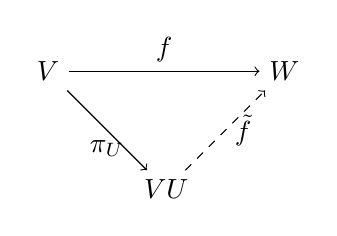
\begin{tikzpicture}
		\node (V) at (0,0) {$V$};
		\node (W) at (3,0) {$W$};
		\node (R) at (1.5,-1.5) {\qraum{$V$}{$U$}};
		\draw[->, above] (V) to node {$f$} (W);
		\draw[->, below] (V)  to node {$\pi_U$} (R);
		\draw[->, right, dashed] (R)  to node {$\tilde f$} (W);
		\end{tikzpicture}
	\end{center}
	Diese erfüllt $\Ker(\tilde f)=$\qraum{$\Ker(f)$}{U}$=\{x+U\mid x\in \Ker(f)\}\subseteq$\qraum{$V$}{$U$}.
\end{theorem}
\begin{proof}
	Ist $f=\tilde f\circ \pi_U$, so gilt $\tilde f(x+U)=\tilde f(\pi_U)=f(x)\; (*)$, somit ist $\tilde f$ dann eindeutig bestimmt. Umgekehrt 
	wird durch $(*)$ eine wohldefinierte Abbildung $\tilde f$ erklärt: Sind $x,x'\in V$ mit $x+U=x'+U$, so ist $x-x'\in U\subseteq \Ker(f)$ und 
	deshalb $f(x)=f(x')$. \\
	\begin{itemize}
		\item Linearität: Für $x,y\in V$ und $\lambda\in K$ ist $\tilde f(\lambda(x+U)+\mu(y+U))=\tilde f(\lambda\pi_U(x)+\mu\pi_U(y))=\lambda\tilde f
		(x+U)+\mu\tilde f(y+U)$.
		\item Kern: $\tilde f(x+U)=0\iff f(x)=0 \iff x\in \Ker(f)$.
	\end{itemize}
\end{proof}

\begin{conclusion}
	\proplbl{3_7_10}
	Für $f\in \Hom_K(V,W)$ ist $\Image(f)\cong $\qraum{$V$}{$\Ker(f)$}. Insbesondere gilt: Ist $f$ ein Epimorphismus, so 
	ist $W\cong $\qraum{$V$}{$\Ker(f)$}.
\end{conclusion}
\begin{proof}
	Betrachte $\tilde f:$\qraum{$V$}{$\Ker(f)$}$\to W$. Nach \propref{3_7_9} ist $\Ker(\tilde f)=$\qraum{$\Ker(f)$}{$\Ker(f)$}$=\{\Ker(f)\}$, 
	also $\tilde f$ injektiv. Nach Definition ist $\tilde f($\qraum{$V$}{$\Ker(f)$}$)=f(V)=\Image(f)$. Somit ist $\tilde f:$\qraum{$V$}
	{$\Ker(f)$}$\to \Image(f)$ ein Isomorphismus.
\end{proof}

\begin{proposition}
	\proplbl{3_7_11}
	Seien $U,U'$ Untervektorraum von $V$. Genau dann ist $V=U\oplus U'$, wenn $\pi_U|_{U'}: U'\to$\qraum{$V$}{$U$} ein Isomorphismus 
	ist.
\end{proposition}
\begin{proof}
	\begin{itemize}
		\item $\pi_U|_{U'}$ injektiv $\iff \Ker(\pi_U|_{U'})=\{0\}\iff \Ker(\pi_U)\cap U'=\{0\}\iff U\cap U'=\{0\}$
		\item $\pi_U|_{U'}$ surjektiv $\iff \forall x\in V \exists u'\in U: \pi_U(u')=\pi_U(x)\iff u'-x\in \Ker(\pi_U)=U\iff x=u+u'\iff V=U+U'$
	\end{itemize}
\end{proof}

\begin{conclusion}
	\proplbl{3_7_12}
	Ist $\dim_K(V)<\infty$, so ist $\dim_K($\qraum{$V$}{$U$}$)=\dim_K(V)-\dim_K(U)$.
\end{conclusion}
\begin{proof}
	Nach \propref{2_4_10} existiert ein lineares Komplement $U'$ zu $U$ in $V$ (d.h. $V=U\oplus U'$) und $\dim_K(U')=\dim_K(V)-\dim_K(U)$. Es gilt \qraum{$V$}
	{$U$}=$U'$.
\end{proof}

\begin{conclusion}
	\proplbl{3_7_13}
	Ist $\dim_K(V)<\infty$ und $f\in \Hom_K(V,W)$, so ist $\dim_K(V)=\dim_K(\Ker(f))+\dim_K(\Image(f))$.
\end{conclusion}
\begin{proof}
	\propref{3_7_11} und \propref{3_7_12}
\end{proof}

\begin{conclusion}
	\proplbl{3_7_14}
	Ist $\dim_K(V)<\infty$ und $f\in \End_K(V)$, so sind äquivalent:
	\begin{itemize}
		\item $f\in \Aut_K(V)$
		\item $f$ ist injektiv
		\item $f$ ist surjektiv
	\end{itemize}
\end{conclusion}
\begin{proof}
	\begin{itemize}
		\item $2\iff \dim_K(\Ker(f))=0$
		\item $3\iff \dim_K(\Image(f))=\dim_K(V)$
	\end{itemize}
\end{proof}

\begin{remark}
	Analog zu dem Quotientenräumen kann man definieren:
	\begin{itemize}
		\item Quotientengruppen \qraum{$G$}{$N$}, wobei $N$ Normalteiler von $G$ ist
		\item Quotientenringe \qraum{$R$}{$I$}, wobei $I$ ein Ideal von $R$ ist (z.B. \qraum{$\mathbb Z$}{$n\mathbb Z$})
	\end{itemize}
	Diese werden in der Vorlesung \textit{Algebra und Zahlentheorie} behandelt.
\end{remark}
\section{Rang}

Seien $V,W$ zwei endlichdimensionale $K$-Vektorräume und $f\in \Hom_K(V,W)$.

\begin{definition}[Rang]
	Der \begriff{Rang} von $f$ ist $\rk(f)=\dim_K(\Image(f))$.
\end{definition}

\begin{remark}
	Nach \propref{3_7_13} ist $\rk(f)=\dim_K(V)-\dim_K(\Ker(f))$. Also ist $f$ genau dann injektiv, wenn $\rk(f)=\dim_K(V)$. Auch sehen wir, 
	dass $\rk(f)\le \min\{\dim_K(V),\dim_K(W)\}$.
\end{remark}

\begin{lemma}
	\proplbl{3_8_3}
	Sei $U$ ein weiterer endlichdimensionaler $K$-Vektorraum und $g\in \Hom_K(U,V)$.
	\begin{itemize}
		\item Ist $g$ surjektiv, dann ist $\rk(f\circ g)=\rk(f)$.
		\item Ist $f$ injektiv, dann ist $\rk(f\circ g)=\rk(g)$.
	\end{itemize}
\end{lemma}
\begin{proof}
	Dies folgt sofort aus $\Image(f\circ g)=f(\Image(g))$.
\end{proof}

\begin{proposition}
	\proplbl{3_8_4}
	Sei $r\in \mathbb N_0$. Genau dann ist $\rk(f)=r$, wenn es $B$ von $V$ und $C$ von $W$ gibt, für die 
	\begin{align}
		M_C^B(f)=E_r&=\sum_{i=1}^r E_{ii}\notag \\ 
		E_r&=\begin{pmatrix}
		1 & 0 & \dots & \dots & \dots & 0 \\
		0 & \ddots & \ddots & \; & \; & \vdots \\
		\vdots & \ddots & 1 & \ddots & \; & \vdots\\
		\vdots & \; & \ddots & 0 & \ddots & \vdots\\
		\vdots & \; & \; & \ddots & \ddots & 0\\
		0 & \dots & \dots & \dots & 0 & 0\\
		\end{pmatrix}\notag
	\end{align}
\end{proposition}
\begin{proof}
	\begin{itemize}
		\item Rückrichtung: Ist $M_C^B(f)=E_r$ und $C=(y_1,...,y_n)$, so ist $\Image(f)=\Span_K(y_1,...,y_r)$, also $\rk(f)=r$.
		\item Hinrichtung: Sei $r=\rk(f)$. Setze $U=\Ker(f)$ und $W=\Image(f)$. Wähle Basis $(y_1,...,y_r)$ und ergänze diese zu einer Basis $C$ von 
		$W$. Wähle für $i=1,...,r$ ein $x_i\in f^{-1}(y_i)$. Dann ist $(x_1,...,x_r)$ linear unabhängig und mit $U'=\Span_K(x_1,...,x_r)$ ist
		$f|_{U'}:U'\to W_0$ ein Isomorphismus nach \propref{3_5_1}. Insbesondere ist $U\cap U'=\{0\}$ und mit \propref{3_7_11} folgt $V=U\oplus U'$. Ist also $(x_{r+1},...,x_n)$ 
		eine Basis von $U$, so ist $B=(x_1,...,x_n)$ eine Basis von $V$ (\propref{2_4_9}). Diese Basis erfüllt $M_C^B(f)=E_r$.
	\end{itemize}
\end{proof}

\begin{definition}[Rang einer Matrix]
	Der Rang einer \begriff[Rang!]{Matrix} $A\in \Mat_{m\times n}(K)$ ist $\rk(A)=\rk(f_A)$, wobei $f_A:K^n\to K^m$ 
	die durch $A$ beschriebene lineare Abbildung ist.
\end{definition}

\begin{mathematica}[Rang einer Matrix]
	Auch für den Rang einer Matrix $A$ hat Mathematica bzw. WolframAlpha eine Funktion
	\begin{align}
		\texttt{MatrixRank[A]}\notag
	\end{align}
\end{mathematica}

\begin{remark}
	\proplbl{3_8_6}
	Sei $A=(a_{ij})\in \Mat_{m\times n}(K)$. Man fasst die Spalten $a_j=(a_{1j},...,a_{mj})^t$ als Elemente des $K^m$ auf 
	und definiert den Spaltenraum $\SR(A)=\Span_K(a_1,...,a_n)\subseteq K^m$. Entsprechend definiert man den Zeilenraum $\ZR(A)=\Span_K(
	\tilde a_1^t,..,\tilde a_m^t)\subseteq K^n$. Es ist $\Image(f_A)=\SR(A)$ und folglich $\rk(A)=\dim_K(\SR(A))$. Außerdem ist $\SR(A^t)=\ZR(A)$ 
	und deshalb $\rk(A^t)=\dim_K(\ZR(A))$. Man nennt $\rk(A)$ deshalb auch den \begriff[Rang!]{Spaltenrang} von $A$ und $\rk(A^t)$ den \begriff[Rang!]{Zeilenrang} von $A$.
\end{remark}

\begin{lemma}
	\proplbl{3_8_7}
	Ist $A\in \Mat_{m\times n}(K)$, $S\in \GL_m(K)$, $T\in \GL_n(K)$, so ist $\rk(SAT)=\rk(A)$.
\end{lemma}
\begin{proof}
	$\rk(SAT)=\rk(f_{SAT})=\rk(f_S\circ f_A\circ f_T)=\rk(f_A)=\rk(A)$, da $f_S$ und $f_T$ bijektiv sind (\propref{3_8_3}).
\end{proof}

\begin{proposition}
	\proplbl{3_8_8}
	Für jedes $A\in \Mat_{m\times n}(K)$ gibt es $S\in \GL_m(K)$ und $T\in \GL_n(K)$ mit $SAT=E_r$, wobei $r=\rk(A)$.
\end{proposition}
\begin{proof}
	Es gibt Basen $B$ von $K^n$ und $C$ von $K^m$ mit $M_C^B(f_A)=E_r$ (\propref{3_8_4}). Mit den Standardbasen $E_n$ bzw. $E_m$ gilt: $M_C^B(f_A)=T_C^{E_m}
	\cdot M_{E_m}^{E_n}(f_A)\cdot (T_B^{E_n})^{-1}=SAT$ mit $S=T_C^{E_m}\in \GL_m(K)$ und $T=(T_B^{E_n})^{-1}\in \GL_n(K)$.
\end{proof}

\begin{conclusion}
	\proplbl{3_8_9}
	Seien $A,B\in \Mat_{m\times n}(K)$. Genau dann gibt es $S\in \GL_m(K)$ und $T\in \GL_n(K)$ mit $B=SAT$, wenn 
	$\rk(A)=\rk(B)$.
\end{conclusion}
\begin{proof}
	\begin{itemize}
		\item Hinrichtung: \propref{3_8_7}
		\item Rückrichtung: $r=\rk(A)=\rk(B)\Rightarrow$ Nach \propref{3_8_8} gibt $S_1,S_2\in \GL_m(K)$ und $T_1,T_2\in \GL_n(K)$ mit $S_1AT_1=E_r=S_2BT_2 \Rightarrow 
		B=S_2^{-1}\cdot SAT_1\cdot T_2^{-1}$.
	\end{itemize}
\end{proof}

\begin{proposition}
	\proplbl{3_8_10}
	Für $A\in \Mat_{m\times n}(K)$ ist $\rk(A)=\rk(A^t)$, anders gesagt: $\dim_K(\SR(A))=\dim_K(\ZR(A))$.
\end{proposition}
\begin{proof}
	Mit \propref{3_8_8} ergibt sich: $SAT=E_r$ mit $r=\rk(A)$, $S\in \GL_m(K)$ und $T\in \GL_n(K)$. Aus $E_r^t=(SAT)^t=T^tA^tS^t$, folgt, 
	dass $\rk(A^t)=\rk(E_r^t)=\rk(A)$.
\end{proof}

\begin{conclusion}
	\proplbl{3_8_11}
	Für $A\in \Mat_n(K)$ sind äquivalent:
	\begin{itemize}
		\item $A\in \GL_n(K)$, d.h. es gibt $S\in \GL_n(K)$ mit $SA=AS=\mathbbm{1}_n$
		\item $\rk(A)=n$
		\item Die Spalten von $A$ sind linear unabhängig.
		\item Die Zeilen von $A$ sind linear unabhängig.
		\item Es gibt $S\in \GL_n(K)$ mit $SA=\mathbbm{1}_n$.
		\item Es gibt $T\in \GL_n(K)$ mit $AT=\mathbbm{1}_n$.
	\end{itemize}
\end{conclusion}
\begin{proof}
	\begin{itemize}
		\item $(1)\iff (2)$: \propref{3_5_11} und \propref{3_7_14}
		\item $(2)\iff (3)$: \propref{3_8_6}
		\item $(2)\iff (4)$: \propref{3_8_6} und \propref{3_8_10}
		\item $(1)\iff (5)\land (6)$: trivial
		\item $(5)\land (6)\iff (2)$: \propref{3_8_9}
	\end{itemize}
\end{proof}
\section{Lineare Gleichungssysteme}

Sei $A\in \Mat_{m\times n}(K)$ und $b\in K^m$.

\begin{definition}[Lineares Gleichungssystem]
	Unter einem \begriff{Linearen Gleichungssystem} verstehen wir eine Gleichung der Form $Ax=b$. 
	Diese heißt \begriff{homogen}, wenn $b=0$, sonst \begriff{inhomogen} und $L(A,b)=\{x\in K^n\mid Ax=b\}$ ist sein \begriff{Lösungsraum}.
\end{definition}

\begin{mathematica}[Lineare Gleichungssysteme]
	Für das Lösen von Linearen Gleichungssystemen gibt es in WolframAlpha bzw. Mathematica verschiedene Verfahren:
	\begin{itemize}
		\item \texttt{Solve[]}:
		\begin{align}
			\texttt{Solve[a == 2 b \&\& b == 5 \&\& c + a == b, \{a, b, c\}]}\notag
		\end{align}
		\item \texttt{LinearSolve[]}: Braucht 2 Argumente: Zum einen die Koeffizientenmatrix $A$ und den Ergebnisvektor $b$. Rückgabe ist dann der Variablenvektor $x$.
		\begin{align}
			\texttt{LinearSolve[\{\{1, 1\}, \{0, 1\}\}, \{6, 10\}]}\notag
		\end{align}
	\end{itemize}
\end{mathematica}

\begin{remark}
	Ist $A=(a_{ij})$, $b=(b_1,...,b_m)^t$, so schreibt man das Lineare Gleichungssystem $Ax=b$ auch
	\begin{align}
	\begin{vmatrix}
		a_{11}x_1 + \dots + a_{1n}x_n & = & b_1\\
		\vdots & \vdots & \vdots\\
		a_{m1}x_1 + \dots + a_{mn}x_n & = & b_m\\
	\end{vmatrix}\notag
	\end{align}
\end{remark}

\begin{remark}
	Das homogene System $Ax=0$ hat als Lösungsraum den Untervektorraum $L(A,0)=\Ker(f_A)$ der Dimension $\dim_K(L(A,0))=n-\rk(A)$. Das 
	inhomogene System hat entweder $L(A,b)=\emptyset$ oder der Lösungsraum ist der affine Unterraum $L(A,b)=f^{-1}(b)=x_0+L(A,0)$, wobei 
	$x_0\in L(A,b)$ beliebig. Man erhält so alle Lösungen des inhomogenen Systems, wenn man eine Lösung und die Lösungen des homogenen 
	Systems kennt.
\end{remark}

\begin{definition}[Zeilenstufenform]
	Die Matrix $A=(a_{ij})$ hat \begriff{Zeilenstufenform}, wenn es ganze Zahlen $0\le r \le m$ und $1\le 
	k_1<...<k_r\le n$ gibt mit:
	\begin{itemize}
		\item für $1\le i \le r$ und $1\le j < k_i$ ist $a_{ij}=0$
		\item für $1\le i \le r$ ist $a_{ik_{i}}\neq 0$ (sogenannte \begriff{Pivotelemente})
		\item für $r<i\le m$ und $1\le j\le n$ ist $a_{ij}=0$
	\end{itemize}
	\begin{align}
		\begin{pmatrix}
		0 & \dots & 0 & a_{1k_{1}} & * & \dots & \dots & *\\
		0 & \dots & \dots & 0 & a_{2k_{2}} & * & \dots & *\\
		\vdots & \vdots & \vdots & \vdots & \vdots & \vdots & \vdots & \vdots\\
		0 & \dots & \dots & \dots & \dots & \dots & \dots & a_{rk_{r}}\\
		0 & \dots & \dots & \dots & \dots & \dots & \dots & 0\\
		\vdots & \; & \; & \; & \; & \; & \; & \vdots\\
		0 & \dots & \dots & \dots & \dots & \dots & \dots & 0\\
		\end{pmatrix}\notag
	\end{align}
\end{definition}

\begin{lemma}
	Sei $A$ in Zeilenstufenform. Dann ist $\rk(A)=r$.
\end{lemma}
\begin{proof}
	Wegen $\rk(A)=\rk(A^t)=\dim_K(\ZR)$ genügt es zu zeigen, dass die ersten $r$ Zeilen $a_1,...,a_r$ linear unabhängig sind. Ist $\sum
	_{i=1}^r \lambda a_i=0$, so ist insbesondere $0=\sum_{i=1}^r \lambda_i a_{ik_{i}}=\lambda_1 a_{1k_{1}}$, also $\lambda_1
	=0$, und dann immer so weiter.
\end{proof}

\begin{proposition}
	\proplbl{3_9_6}
	Sei $A$ in Zeilenstufenform.
	\begin{itemize}
		\item Ist $b_i\neq 0$ für ein $r<i\le m$, so ist $L(A,b)=\emptyset$.
		\item Ist $b_i=0$ für alle $r<i\le m$, so erhält man alle $x\in L(A,b)$, indem man erst $x_j\in K$ für $j\in \{1,..,n\}
		\backslash \{k_1,...,k_r\}$ beliebig wählt und dann für $i=r,r-1,...,1$ rekursiv $x_{k_{i}}=a_{1k_{i}}^{-1}\cdot (b_i-\sum
		_{j=k_i+1}^n a_{ij}\cdot x_j)\quad (*)$ setzt.
	\end{itemize}
\end{proposition}
\begin{proof}
	\begin{itemize}
		\item Klar.
		\item Sicher erhält man auf diese Weise Lösungen $x\in L(A,b)$. Umgekehrt muss jede solche Lösung $(*)$ erfüllen, man erhält auf 
		diese Weise also alle.
	\end{itemize}
\end{proof}

\begin{definition}[Elementarmatrizen]
	Für $i,j\in \{1,...,m\}$, $\lambda \in K^{\times}$ und $\mu\in K$ definieren wir 
	$m\times m$-Matrizen, die sogenannten \begriff{Elementarmatrizen}:
	\begin{itemize}
		\item $S_i(\lambda):=\mathbbm{1}_m + (\lambda-1)E_{ii}$
		\item $Q_{ij}(\mu):= \mathbbm{1}_m + \mu E_{ij}$
		\item $P_{ij}:= \mathbbm{1}_m + E_{ij} + E_{ji} - E_{ii} - E_{jj}$
	\end{itemize}
\end{definition}

\begin{remark}
	Multiplikation einer dieser Matrizen von links an die Matrix $A$ hat folgende Wirkung:
	\begin{itemize}
		\item $S_i(\lambda)\cdot A$: Multiplikation der $i$-ten Zeile mit $\lambda$
		\item $Q_{ij}(\mu)\cdot A$: Addition des $\mu$-fachen der $j$-ten Zeile zur $i$-ten Zeile
		\item $P_{ij}$: Vertauschung von $i$-ter und $j$-ter Zeile
	\end{itemize}
	Man spricht dann von sogenannten elementaren Zeilenumformungen der Matrix $A$ von Typ I, II oder III.
\end{remark}

\begin{lemma}
	Es sind $S_i(\lambda),Q_{ij}(\mu),P_{ij}\in \GL_m(K)$. Dann ist $S_i(\lambda)^{-1}=S_i(\lambda^{-1}), Q_{ij}(\mu)
	^{-1}=Q_{ij}(-\mu),P_{ij}^{-1}=P_{ij}$. Insbesondere gilt: Ist $E$ eine der Elementarmatrizen, so ist $\ZR(EA)=\ZR(A)$ und $L(EA,0)=
	L(A,0)$. Weiterhin ist $\rk(EA)=\rk(A)$.
\end{lemma}
\begin{proof}
	Inverse nachprüfen. Da $E\in \GL_m(K)$ sind $f_E,f_{E^t}\in Aut_K(K^m)$, also $\ZR(EA)=\SR((EA)^t)=\Image(f_{A^tE^t})=\Image(f_{A^t}\circ
	f_{E^t})=\Image(f_{A^t})=\ZR(A)$ und $L(EA,0)=\Ker(f_{EA})=\Ker(f_E\circ f_A)=\Ker(f_A)=L(A,0)$.
\end{proof}

\begin{remark}
	Anders gesagt: Elementare Zeilenumformungen verändern den Lösungsraum eines homogenen linearen Gleichungssystems 
	nicht.
\end{remark}

\begin{theorem}[Eliminierungsverfahren nach \person{Gauß}]
	\proplbl{3_9_11}
	Zu jeder Matrix $A\in \Mat_{m\times n}(K)$ gibt es $l\in \mathbb N_0$ und 
	Elementarmatrizen $E_1,...,E_l$ vom Typ II und III für die $E_l\cdot ... \cdot E_1\cdot A$ in Zeilenstufenform ist. 
\end{theorem}
\begin{proof}
	Seien $a_1,...,a_n$ die Spalten von $A$. \\
	Ist $A=0$ so ist nichts zu tun. \\
	Sei nun $A\neq 0$ und sei $k_1$ minimal mit $a_{k_1}\neq 0$. Es gibt also ein $i$ mit $a_{ik_1}\neq 0$. Durch Vertauschen der ersten 
	und der $i$-ten Zeile erreichen wir, dass $a_{1k_1}=0$, d.h. wir multiplizieren $A$ mit $E_1=P_{1i}$. Nun addieren wir für $i=2,..,m$ 
	ein geeignetes Vielfaches der ersten Zeile zur $i$-ten Zeile, um $a_{ik_1}=0$, d.h. wir multiplizieren $A$ mit $E_i=Q_{i1}(\mu_i)$ für 
	$\mu_i=\frac{a_{ik_1}}{a_{1k_1}}$. Nach diesen Umformungen haben wir eine Matrix der Form:
	\begin{align}\begin{pmatrix}
		0 & \dots & 0 & a_{1k_1} & * & \dots & *\\
		0 & \dots & \dots & 0 & \textcolor{red}{*} & \textcolor{red}{\dots} & \textcolor{red}{*}\\
		\vdots & \vdots & \vdots & \vdots & \textcolor{red}{\vdots} & \textcolor{red}{\vdots} & \textcolor{red}{\vdots}\\
		0 & \dots & \dots & 0 & \textcolor{red}{*} & \textcolor{red}{\dots} & \textcolor{red}{*}\\
		\end{pmatrix}\notag\end{align}
	und können nun mit dem \textcolor{red}{Rest der Matrix $A=:A'$} von vorne beginnen. Die nun folgenden Zeilenumformungen werden die 
	erste Zeile und die ersten $k_1$ Spalten nicht mehr ändern, und weil $A'$ weniger Zeilen und Spalten als $A$ hat, bricht das Verfahren 
	nach endlich vielen Schritten ab.
\end{proof}

\begin{mathematica}[\person{Gauss}-Verfahren]
	Auch für das \person{Gauss}-Verfahren hat Mathematica bzw. WolframAlpha eine Funktion. Sie gibt die Matrix nach Ausführung des \person{Gauss}-Algorithmus zurück.
	\begin{align}
		\texttt{RowReduce[\{\{1, 4\}, \{2, 5\}\}]}\notag
	\end{align}
\end{mathematica}

\begin{conclusion}
	Zu jeder Matrix $A$ gibt es eine invertierbare Matrix $S\in \GL_n(K)$ für die $SA$ in Zeilenstufenform ist.
\end{conclusion}
\begin{proof}
	folgt direkt aus \propref{3_9_11} mit $S=E_l\cdot ... \cdot E_1$
\end{proof}

\begin{remark}
	Der Beweis für das Eliminierungsverfahren (\propref{3_9_11}) liefert ein Verfahren, die Elementarmatrizen $E_1,...,E_l$ zu finden. 
	Damit erhält man ein Verfahren ein lineares Gleichungssystem zu lösen. Setzt man $S=E_l\cdot ... \cdot E_1$, $A'=SA$ und $b'=Sb$, so 
	ist $L(A,b)=L(A',b')$: $Ax=b\Rightarrow SAx=Sb$ bzw. $A'x=b' \Rightarrow S^{-1}A'x=S^{-1}b'$. \\
	Das Gleichungssystem kann dann mit \propref{3_9_6} gelöst werden. Praktisch führt man die elementaren Zeilenumformungen an $A$ parallel dazu auch an $b$ 
	durch.
\end{remark}

\begin{remark}
	Es gibt von diesem Verfahren verschiedene Varianten und weitere Anwendungen: So kann man z.B. die Invertierbarkeit 
	einer Matrix $A\in \Mat_n(K)$ prüfen und ggf. das Inverse bestimmen: Ist $E_l\cdot ... \cdot E_1\cdot A$ in Zeilenstufenform, so ist $A$ 
	genau dann invertierbar, wenn alle Zeilen von Null verschieden sind. Ist dies der Fall, so ist $r=n$ und $k_i=i$ für alle $i$, 
	und man findet weitere Elementarmatrizen $E_{l+1},...,E_s$ vom Typ I und II, für die $E_s\cdot ... \cdot E_1\cdot A=\mathbbm{1}_n$. Dann ist 
	$S'=E_s\cdot ... \cdot E_1\cdot A=A^{-1}$ (vgl. \propref{3_8_11}). Praktisch erhält man $A^{-1}$, indem man die Zeilenumformungen an $A$ parallel dazu 
	auch an $\mathbbm{1}_n$ ausführt.
\end{remark}

\begin{conclusion}
	Jedes $A\in \GL_m(K)$ ist ein Produkt von Elementarmatrizen.
\end{conclusion}
\begin{proof}
	$A^{-1}=S'=E_s\cdot ... \cdot E_1 \Rightarrow A=(E_s\cdot ... \cdot E_1)^{-1}=E_1^{-1}\cdot ... \cdot E_s^{-1}$
\end{proof}

\chapter{Determinanten}
\section{Das Vorzeichen einer Permutation}
\section{Determinante einer Matrix}

\begin{definition}[Determinantenabbildung]
	Eine Abbildung $\delta:\Mat_n(R)\to R$ heißt \begriff{Determinantenabbildung}, wenn gilt:
	\begin{itemize}
		\item (D1): $\delta$ ist linear in jeder Zeile: sind $a_1,...,a_n$ die Zeilen von $A$ und ist $i\in \{1,...,n\}$ und $a_i=\lambda'a'_i + 
		\lambda''a''_i$ mit $\lambda',\lambda''\in R$ und den Zeilenvektoren $a'_i,a''_i$, so ist $\delta(A)=\lambda'\cdot \delta(a_1,...,
		a'_i,...,a_n) + \lambda''\cdot \det(a_1,...,a''_i,...,a_n)$.
		\item (D2): $\delta$ ist alternierend: sind $a_1,...,a_n$ die Zeilen von $A$ und $i,j\in \{1,...,n\}$, $i\neq j$ mit $a_i=a_j$, so ist 
		$\delta(A)=0$.
		\item (D3): $\delta$ ist normiert: $\delta(\mathbbm{1}_n)=1$.
	\end{itemize}
\end{definition}

\begin{theorem}
	\proplbl{4_2_8}
	Es gibt genau eine Determinantenabbildung $\delta:\Mat_n(R)\to R$ und diese ist gegeben durch die 
	Leibnitzformel 
	\begin{align}
		\det(a_{ij})=\sum_{\sigma\in S_n} \sgn(\sigma)\cdot \prod_{i=1}^n a_{i,\sigma(i)} = \sum_{\sigma
			\in A_n}\prod_{i=1}^n a_{i,\sigma(i)} - \sum_{\sigma\in S_n\backslash A_n}\prod_{i=1}^n a_{i,\sigma(i)}\notag
	\end{align}
\end{theorem}
\begin{proof}
	Eindeutigkeit der Abbildung folgt wegen D3 aus \propref{4_2_7}. Bleibt nur noch zu zeigen, dass $\det$ auch die Axiome D1 bis D3 erfüllt. \\
	D1: klar \\
	D3: klar \\
	D2: Seien $\mu\neq v$ mit $a_{\mu}=a_v$. Mit $\tau=\tau_{\mu v}$ ist $S_n\backslash A_n = A_n\tau$, somit 
	\begin{align}
		\det(a_{ij})&=
		\sum_{\sigma\in A_n} \prod_{i=1}^n a_{i,\sigma(i)}-\sum_{\sigma\in A_n\tau} \prod_{i=1}^n a_{i,\sigma\tau(i)} \notag \\
		&=
		\sum_{\sigma\in A_n} \left( \prod_{i=1}^n a_{i,\sigma(i)} - \prod_{i=1}^n a_{i,\sigma\tau(i)} \right) \notag
	\end{align}
	nach \propref{4_1_10}. Da $a_{ij}=a_{\tau(i),j}$ 
	für alle $i,j$ ist 
	\begin{align}
		\prod_{i=1}^n a_{i,\sigma(i)}&=\prod_{i=1}^n a_{\tau(i),\sigma\tau(i)} \notag \\
		&=\prod_{i=1}^n a_{i,\sigma\tau(i)} \notag
	\end{align}
	für jedes $\sigma\in S_n$, woraus $\det(a_{ij})=0$ folgt.
\end{proof}

\begin{theorem}[Determinantenmultiplikationssatz]
	\proplbl{4_2_11}
	Für $A,B\in \Mat_n(R)$ ist 
	\begin{align}
		\det(AB)=\det(A)\cdot \det(B)\notag
	\end{align}
\end{theorem}
\begin{proof}
	Fixiere $A$ und betrachte die Abbildung $\delta: \Mat_n(R)\to R$ mit $B\mapsto \det(AB^{-1})$. Diese Abbildung erfüllt die Axiome 
	D1 und D2. sind $b_1,...,b_n$ die Zeilen von $B$, so hat $AB^{-1}$ die Spalten $Ab_1^t,...,Ab_n^t$, es werden die Eigenschaften 
	von $\det$ auf $\delta$ übertragen. \\
	$\Rightarrow \det(AB)=\delta(B^t)=\delta(\mathbbm{1}_n)\cdot \det(B^t)=\det(A)\cdot \det(B)$.
\end{proof}
\section{Minoren}

Seien $m,n\in \mathbb N$.

\begin{definition}[adjungierte Matrix]
	Sei $A=(a_{ij})\in \Mat_n(R)$. Für $i,j\in \{1,...,n\}$ definieren wir die $n\times n$-Matrix: \\
	\begin{align}
		A_{ij}=\begin{pmatrix}
		a_{11} & ... & a_{1,j-1} & 0 & a_{1,j+1} & ... & a_{1n} \\
		\vdots & \ddots & \vdots & \vdots & \vdots & \ddots & \vdots \\
		a_{i-1,1} & ... & a_{i-1,j.1} & 0 & a_{i-1,j+1} & ... & a_{i-1,n} \\
		0 & ... & 0 & 1 & 0 & ... & 0 \\
		a_{i+1,1} & ... & a_{i+1,j.1} & 0 & a_{i+1,j+1} & ... & a_{i+1,n} \\
		\vdots & \ddots & \vdots & \vdots & \vdots & \ddots & \vdots \\
		a_{n1} & ... & a_{n,j-1} & 0 & a_{n,j+1} & ... & a_{nn} \\
		\end{pmatrix}\notag
	\end{align}
	die durch Ersetzen der $i$-ten Zeile und der $j$-ten Spalte durch $e_j$ aus $A$ hervorgeht, sowie die $(n-1)\times(n-1)$-
	Matrix: \\
	\begin{align}
		A'_{ij}=\begin{pmatrix}
		a_{11} & ... & a_{1,j-1} & a_{1,j+1} & ... & a_{1n} \\
		\vdots & \ddots & \vdots & \vdots & \ddots & \vdots \\
		a_{i-1,1} & ... & a_{i-1,j.1} & a_{i-1,j+1} & ... & a_{i-1,n} \\
		a_{i+1,1} & ... & a_{i+1,j.1} & a_{i+1,j+1} & ... & a_{i+1,n} \\
		\vdots & \ddots & \vdots & \vdots & \ddots & \vdots \\
		a_{n1} & ... & a_{n,j-1} & a_{n,j+1} & ... & a_{nn} \\
		\end{pmatrix}\notag
	\end{align}
	die durch Streichen der $i$-ten Zeile und der $j$-ten Spalten entsteht. Weiterhin definieren wir die zu $A$ \begriff{adjungierte Matrix} 
	als $A^\#=(a_{ij}^\#)\in \Mat_n(R)$, wobei $a_{ij}^\#=\det(A_{ji})$.
\end{definition}

\begin{lemma}
	\proplbl{4_3_2}
	Sei $A\in \Mat_n(R)$ mit Spalten $a_1,...,a_n$. Für $i,j\in \{1,..,n\}$ gilt:
	\begin{itemize}
		\item $\det(A_{ij})=(-1)^{i+j}\cdot \det(A'_{ij})$
		\item $\det(A_{ij})=\det(a_1,...,a_{j-1},e_i,a_{j+1},...,a_n)$
	\end{itemize}
\end{lemma}
\begin{proof}
	\begin{itemize}
		\item Durch geeignete Permutation der ersten $i$ Zeilen und der ersten $j$ Zeilen erhält man 
		\begin{align}
			\det(A_{ij})&=(-1)^{(i-1)+
				(j-1)} \cdot \det(\begin{pmatrix}1&0&...&0 \\ 0 & \; & \; & \; \\ \vdots & \; & A'_{ij} & \; \\ 0 & \; & \; & \; \\ \end{pmatrix})\notag \\
			&\overset{\propref{4_2_9}}{=}(-1)^{i+j}\cdot \det(\mathbbm{1}_n)\cdot \det(A'_{ij})\notag
		\end{align}
		\item Man erhält $A_{ij}$ aus $(a_1,...,e_i,...,a_n)$ durch elementare Spaltenumformungen vom Typ II.
	\end{itemize}
\end{proof}

\begin{proposition}
	\proplbl{4_3_3}
	Für $A\in \Mat_n(R)$ ist 
	\begin{align}
		A^\#\cdot A=A\cdot A^\#=\det(A)\cdot \mathbbm{1}_n \notag
	\end{align}
\end{proposition}
\begin{proof}
	\begin{align}
		(A^\#A)_{ij}&=\sum_{k=1}^n a^\#_{ik}\cdot a_{kj} \notag \\
		&=\sum_{k=1}^n a_{kj}\cdot \det(A_{kj}) \notag \\
		&\overset{\propref{4_3_2}}{=}\sum_{k=1}^n a_{kj}\cdot \det(a_1,...,a_{i-1},a_j,a_{i+1},...,a_n) \notag \\
		&=\det(a_1,...,a_{i-1},\sum_{k=1}^n a_{kj}e_k,a_{i+1},...,a_n) \notag \\
		&= \det(a_1,...,a_{i-1},a_j,a_{i+1},...,a_n) \notag \\
		&=\delta_{ij}\cdot \det(A) \notag \\
		&=(\det(A)\cdot \mathbbm{1}_n)_{ij} \notag
	\end{align}
	Analog bestimmt man die Koeffizienten von $AA^\#$, wobei man 
	$\det(A_{jk})=\det(A_{jk}^t)=\det((A^t)_{kj})$ benutzt.
\end{proof}

\begin{conclusion}
	\proplbl{4_3_4}
	Es ist $\GL_n(R)=\{A\in \Mat_n(R) \mid \det(A)\in R^{\times}\}$ und für $A\in \GL_n(R)$ ist $A^{-1}=
	\frac{1}{\det(A)}\cdot A^\#$.
\end{conclusion}
\begin{proof}
	\propref{4_3_3} und \propref{4_2_12}
\end{proof}

\begin{proposition}[\person{Laplace}'scher Entwicklungssatz]
	Sei $A=(a_{ij})\in \Mat_n(R)$. Für jedes $i,j\in \{1,..,n\}$ gilt die 
	Formel für die Entwicklung nach der $i$-ten Zeile:
	\begin{align}
		\det(A)=\sum_{j=1}^n (-1)^{i+j}\cdot a_{ij}\cdot \det(A'_{ij})\notag
	\end{align}
	Gleiches gilt auch für Spalten.
\end{proposition}
\begin{proof}
	Nach \propref{4_3_3} ist
	\begin{align}
		\det(A)=(AA^\#)_{ij}&=\sum_{j=1}^n a_{ij}\cdot a^\#_{ij} \notag \\
		&= \sum_{j=1}^n a_{ij}\cdot \det(A_{ij}) \notag \\
		&=\sum_{j=1}^n a_{ij}\cdot (-1)^{i+j}\cdot \det(A'_{ij}) \notag
	\end{align}
	Analog auch für Spalten.
\end{proof}

\begin{proposition}[\person{Cramer}'sche Regel]
	Sei $A\in \GL_n(R)$ mit Spalten $a_1,...,a_n$ und sei $b\in R^n$. Weiter sei 
	$x=(x_1,...,x_n)^t\in R^n$ die eindeutige Lösung des Linearen Gleichungssystems $Ax=b$. Dann ist für $i=1,...,n$ 
	\begin{align}
		x_i=\frac{\det(a_1,...,a_{i-1},b,a_{i+1},...,a_n)}{\det(A)}\notag
	\end{align}
\end{proposition}
\begin{proof}
	\begin{align}
		x_i&=(A^{-1}b)_i \notag \\
		&=\sum_{j=1}^n (A^{-1})_{ij}\cdot b_j \notag \\
		&\overset{\propref{4_3_4}}{=}\frac{1}{\det(A)}\cdot \sum_{j=1}^n a^\#_{ij}\cdot b_j  \notag \\
		&\overset{\propref{4_3_2}}{=} \frac{1}{\det(A)}\cdot \sum_{j=1}^n b_j\cdot\det(a_1,...,a_{i-1},e_i,a_{i+1},...,a_n) \notag \\
		&=\frac{1}{\det(A)}\cdot \det(a_1,...,a_{i-1},b_j,a_{i+1},...,a_n) \notag
	\end{align}
\end{proof}

\begin{definition}[Minor]
	Sei $A=(a_{ij})\in \Mat_{m\times n}(R)$ und $1\le r \le m$, $1\le s \le n$. Eine $r\times s$-
	Teilmatrix von $A$ ist eine Matrix der Form $(a_{i\mu,jv})_{\mu,v}\in \Mat_{r\times s}(R)$ mit $1\le i_1<...<i_r\le m$ 
	und $1\le j_1<...<j_s\le n$. Ist $A'$ eine $r\times r$-Teilmatrix von $A$, so bezeichnet man $\det(A')$ als einen 
	$r$-\begriff{Minor} von $A$.
\end{definition}

\begin{example}
	Ist $A\in \Mat_n(R)$ und $i,j\in \{1,...,n\}$, so ist $A'_{ij}$ eine Teilmatrix und $\det(A'_{ij})=(-1)^{i+j}
	\cdot a^\#_{ji}$ ein $(n-1)$-Minor von $A$.
\end{example}

\begin{proposition}
	Sei $A\in \Mat_n(R)$ und $r\in \mathbb N$. Genau dann ist $\rk(A)\ge r$, wenn es eine $r\times r$-
	Teilmatrix $A'$ von $A$ mit $\det(A^{\prime})\neq 0$ gibt.
\end{proposition}
\begin{proof}
	\begin{itemize}
		\item Hinrichtung: Ist $\rk(A)\ge r$, so hat $A$ $r$ linear unabhängige Spalten $a_1,...,a_r$. Die Matrix $\tilde A=(a_1,...,a_r)$ 
		hat den Rang $r$ und deshalb $r$ linear unabhängige Zeilen $\widetilde{a_1},...,\widetilde{a_r}$. Die $r\times r$-Matrix $A$ hat 
		dann Rang $r$, ist also invertierbar, und $\det(A)\neq 0$.
		\item Rückrichtung: Ist $A'$ eine $r\times r$-Teilmatrix von $A$ mit $\det(A')\neq 0$, so ist $\rk(A)\ge \rk(A')=r$.
	\end{itemize}
\end{proof}

\begin{conclusion}
	Sei $A\in \Mat_{m\times n}(K)$. Der Rang von $A$ ist das größte $r\in \mathbb N$, für das 
	$A$ einen von Null verschiedenen $r$-Minor hat.
\end{conclusion}
\section{Determinante und Spur von Endomorphismen}

Sei $n\in \mathbb N$ und $V$ ein $K$-Vektorraum mit $\dim_K(V)=m$.

\begin{proposition}
	\proplbl{4_4_1}
	Sei $f\in \Hom_K(V,W)$, $A'$ eine Basis von $V$ und $A=M_{A'}(f)$. Sei weiter $B\in \Mat_n(K)$. Genau 
	dann gibt es eine Basis $B'$ von $V$ mit $B=M_{B'}(f)$, wenn es $S\in \GL_n(K)$ mit $B=SAS^{-1}$ gibt.
\end{proposition}
\begin{proof}
	Ist $B'$ eine Basis von $V$ mit $B=M_{B'}(f)$, so ist $B=SAS^{-1}$ mit $S=T^{A'}_{B'}$. Sei umgekehrt $B=SAS^{-1}$ mit 
	$S\in \GL_n(K)$. Es gibt eine Basis $B'$ von $V$ mit $T^{A'}_{B'}=S$, also $M_{B'}(f)=T^{A'}_{B'}\cdot M_{A'}(f)\cdot (
	T^{A'}_{B'})^{-1}=SAS^{-1}=B$: Mit $B'=(\Phi_{A'}(f_s^{-1}(e_1)),...,\Phi_{A'}(f_s^{-1}(e_n)))$ ist $\Phi_{A'}\circ f_s^{-1}=
	\id_V\circ \Phi_{B'}$, also $T^{A'}_{B'}=M_{A'}^{A'}(\id_V)=S^{-1}$. Folglich ist $T^{A'}_{B'}=(T_{A'}^{B'})^{-1}=(S^{-1})^{-1}
	=S$ nach \propref{3_6_2}.
\end{proof}

\begin{definition}[Ähnlichkeit]
	Zwei Matrizen $A,B\in \Mat_n(R)$ heißen \begriff{ähnlich}, wenn (in Zeichen $A\sim B$) es 
	$S\in \GL_n(R)$ mit $B=SAS^{-1}$ gibt.
\end{definition}

\begin{proposition}
	Ähnlichkeit von Matrizen ist eine Äquivalenzrelation auf $\Mat_n(R)$.
\end{proposition}
\begin{proof}
	\begin{itemize}
		\item Reflexivität: $A=\mathbbm{1}_n\cdot A \cdot (\mathbbm{1}_n)^{-1}$
		\item Symmetrie: $B=SAS^{-1}\Rightarrow A=S^{-1}BS=S^{-1}B(S^{-1})^{-1}$
		\item Transitivität: $B=SAS^{-1}$, $C=TBT^{-1}\Rightarrow C=TSAS^{-1}T^{-1}=(TS)A(ST)^{-1}$
	\end{itemize}
\end{proof}

\begin{proposition}
	\proplbl{4_4_4}
	Seien $A,B\in \Mat_n(R)$. Ist $A\sim B$, so ist
	\begin{align}
		\det(A)=\det(B)\notag
	\end{align}
\end{proposition}
\begin{proof}
	$B=SAS^{-1}$, $S\in \GL_n(R)$, $\det(B)=\det(S)\cdot \det(A)\cdot \det(S)^{-1}=\det(A)$ nach \propref{4_2_11} und \propref{4_2_12}
\end{proof}

\begin{definition}[Determinante eines Endomorphismus]
	Die \begriff[Endomorphismus!]{Determinante} eines Endomorphismus $f\in \End_K(V)$ ist 
	\begin{align}
		\det(f)=\det(M_B(f))\notag
	\end{align}
	wobei $B$ eine Basis von $V$ ist. (Diese ist wohldefiniert nach \propref{4_4_1} und \propref{4_4_4})
\end{definition}

\begin{proposition}
	\proplbl{4_4_6}
	Für $f,g\in \End_K(V)$ gilt:
	\begin{itemize}
		\item $\det(\id_V)=1$
		\item $\det(f\circ g)=\det(f)\cdot \det(g)$
		\item Genau dann ist $\det(f)\neq 0$, wenn $f\in \Aut_K(V)$. In diesem Fall ist $\det(f^{-1})=\det(f)^{-1}$
	\end{itemize}
\end{proposition}
\begin{proof}
	\begin{itemize}
		\item klar
		\item folgt aus \propref{3_6_6} und \propref{4_2_11}
		\item folgt aus \propref{3_6_5} und \propref{4_2_12}
	\end{itemize}
\end{proof}

\begin{definition}[Spur einer Matrix]
	Die \begriff[Matrix!]{Spur} einer Matrix $A=(a_{ij})\in \Mat_n(R)$ ist 
	\begin{align}
		\tr(A)=\sum_{i=1}^n a_{ii}\notag
	\end{align}
\end{definition}

\begin{mathematica}[Spur einer Matrix]
	Auch für die Spur einer Matrix hat Mathematica bzw. WolframAlpha eine Funktion:
	\begin{align}
		\texttt{Tr[\{\{1, 2, 3\}, \{4, 5, 6\}, \{7, 8, 9\}\}]}\notag
	\end{align}
\end{mathematica}

\begin{lemma}
	\proplbl{4_4_8}
	Seien $A,B\in \Mat_n(R)$
	\begin{itemize}
		\item $\tr: \Mat_n(R)\to R$ ist $R$-linear
		\item $\tr(A^t)=\tr(A)$
		\item $\tr(AB)=\tr(BA)$
	\end{itemize}
\end{lemma}
\begin{proof}
	in den Übungen bereits behandelt
\end{proof}

\begin{proposition}
	\proplbl{4_4_9}
	Seien $A,B\in \Mat_n(R)$. Ist $A\sim B$, so ist $\tr(A)=\tr(B)$.
\end{proposition}
\begin{proof}
	$B=SAS^{-1}$, $S\in \GL_n(R)\Rightarrow \tr(B)=\tr(SAS^{-1})\overset{\propref{4_4_8}}{=}\tr(AS^{-1}S)=\tr(A)$
\end{proof}

\begin{definition}[Spur eines Endomorphismus]
	Die \begriff[Endomorphismus!]{Spur} eines Endomorphismus $f\in \End_K(V)$ ist
	\begin{align}
		\tr(f)=\tr(M_B(f))\notag
	\end{align} 
	wobei $B$ eine Basis von $V$ ist (Diese ist wohldefiniert nach \propref{4_4_1} und \propref{4_4_9})
\end{definition}

\begin{remark}
	Im Fall $K=\mathbb R$ kann man wie in \propref{4_2_3} den Absolutbetrag der Determinante eines $f\in \End_K(K^n)$ 
	geometrisch interpretieren, nämlich als das Volumen von $f(Q)$, wobei $Q=[0,1]^n$ der Einheitsquader ist, und somit 
	als Volumenänderung durch $f$. Auch das Vorzeichen von $\det(f)$ hat eine Bedeutung: Es gibt an, ob $f$ 
	orientierungserhaltend ist. Für erste Interpretationen der Spur siehe A100.
\end{remark}

\part*{Anhang}
\addcontentsline{toc}{part}{Anhang}
\appendix

\chapter{Listen}
\section{Liste der Theoreme}
\theoremlisttype{allname}
\listtheorems{theorem}

\pagebreak
\section{Liste der benannten Sätze}
\theoremlisttype{optname}
\listtheorems{proposition, lemma}

\pagebreak
\section{Liste der Mathematica/WolframAlpha-Befehle}
\smiley{} für faule Mathematiker \smiley{} \\
\theoremlisttype{allname}
\listtheorems{mathematica}

%\printglossary[type=\acronymtype]

\printindex

\end{document}
